% standard
\documentclass[a4paper,11pt]{article}
\usepackage[utf8]{inputenc}
\usepackage[ngerman]{babel}

\usepackage{titlesec}

\setcounter{secnumdepth}{5}
\setcounter{tocdepth}{5}
\titleformat{\paragraph} {\normalfont\normalsize\bfseries}{\theparagraph}{1em}{}
\titlespacing*{\paragraph}
{0pt}{3.25ex plus 1ex minus .2ex}{1.5ex plus .2ex}

%for linkt page numbers in table f content
\usepackage[linktocpage=true]{hyperref}

\hypersetup{%
unicode,pdffitwindow,
pdfkeywords = {pdf, LaTeX, hyperref, thumbnails}, 
pdfauthor = {Brüder Grimm},
bookmarksopen = true,
bookmarksnumbered = true,
pdfcenterwindow=true,
pdffitwindow = true,
pdfstartview=FitBV,
pdfcreator = {pdflatex},
colorlinks=true, breaklinks=true, %
urlcolor=magenta, % color for \url
filecolor=cyan, % color for file
linkcolor=black, % color for \ref
citecolor=magenta, %color for \cite
menucolor=darkblue,
breaklinks=true,anchorcolor=green
}

% for the Glossar
\usepackage{glossaries}
\renewcommand*{\glstextformat}[1]{\textcolor{blue}{#1}}

% für Listings für Java
\usepackage{listings}
%lstset{numbers=left, %
% numberstyle=\tiny, %
% numbersep=5pt, %
% keywordstyle=\color{black}\bfseries, %
% stringstyle=\ttfamily, %
% showstringspaces=false, %
% basicstyle=\footnotesize, %
% captionpos=b}
%lstset{language=java}

% geometry
\usepackage{geometry}
\geometry{ headsep=20pt,
headheight=20pt,
left=21mm,
top=15mm,
right=21mm,
bottom=15mm,
footskip=20pt,
includeheadfoot}

% for using wrapfigures
\usepackage{wrapfig}

% header and footer
\usepackage{datetime}
\newdateformat{dmy}{%
\THEDAY.~\monthname[\THEMONTH] \THEYEAR}
\usepackage{fancyhdr}
\pagestyle{fancy}
\lhead{Noah Vogt \& Simon Hammer}
\chead{}
%\rhead{\dmy\today}
\lfoot{}
\cfoot{Gymnasium Kirschgarten}
\rfoot{Seite \thepage}
\renewcommand{\footrulewidth}{.4pt}

% fix figure positioning
\usepackage{float}

% larger inner table margin
\renewcommand{\arraystretch}{1.4}

% no paragraph indent
\setlength{\parindent}{0em}

\usepackage{comment}

% graphics package
\usepackage{graphicx}

\usepackage{multicol}

\usepackage{multirow}

% use sans serif font
\usepackage{tgheros}
\usepackage{mathptmx}

% don't even ask what this is for, I have no idea (noah)
\usepackage{bm} %italic \bm{\mathit{•}}
\usepackage[hang]{footmisc}
\usepackage{siunitx}
\usepackage[font={small,it}]{caption}
\sisetup{locale = DE, per-mode = fraction, separate-uncertainty,   exponent-to-prefix, prefixes-as-symbols = false, scientific-notation=false
}
\newcommand{\ns}[4]{(\num[scientific-notation=false]{#1}\pm\num[scientific-notation=false]{#2})\cdot\num[]{e#3}\si{#4}}

% show isbn in bibliography
% \usepackage{natbib}

% for quotes
\newenvironment{nicequote}[2]{
    \begin{center}\begin{quote}\textit{#1}\\\par\raggedleft--- {#2}
    }{
    \end{quote}\end{center}
}

\makeindex

% using \say{} for easier quoting
\usepackage{dirtytalk}

% for code snippits
\usepackage{listings}
\usepackage{color}

\definecolor{dkgreen}{rgb}{0,0.6,0}
\definecolor{gray}{rgb}{0.5,0.5,0.5}
\definecolor{mauve}{rgb}{0.58,0,0.82}
\definecolor{background}{rgb}{0.36,0.36,0.36}

% define java code snippit style
%\lstset{frame=tb,
  %language=Java,
  %aboveskip=3mm,
  %belowskip=3mm,
  %showstringspaces=false,
  %columns=flexible,
  %basicstyle={\small\ttfamily},
  %numbers=none,
  %numberstyle=\tiny\color{gray},
  %keywordstyle=\color{blue},
  %commentstyle=\color{dkgreen},
  %stringstyle=\color{mauve},
  %breaklines=true,
  %breakatwhitespace=true,
  %tabsize=3
%}
\lstset{
    numbersep=3pt,
    keywordstyle=\color{blue},
    commentstyle=\color{dkgreen},
    stringstyle=\color{mauve},
    backgroundcolor = \color{background},
    breaklines=true,
    numbers=left,
    numberstyle=\scriptsize\color{black},
    frame=none,
    basicstyle = \small\ttfamily,
    breaklines=true
    breakatwhitespace=false,
    columns=flexible,
    xleftmargin=0.5cm,framesep=8pt,framerule=0pt,
    aboveskip=3mm,
    belowskip=3mm,
}

%\usepackage[backend=biber,style=apa]{biblatex}
\usepackage[
backend=biber,
style=alphabetic,
sorting=ynt
]{biblatex}
\addbibresource{lit/refs.bib}

%========================Glossaries======================

\makeglossaries

\newglossaryentry{copyleft}{
    name=Copyleft-Softwarelizenzen,
    description={Wie bei permissiven Lizenzen können Sie das Programm für JEDEN Zweck ausführen, den Quellcode lesen, ändern und die Änderungen zu veröffentlichen. Der Trick liegt jedoch in den restriktiven Redistributionsbedingungen: Sie dürfen das Programm NUR verbreiten, wenn Ihre Version die gleichen Freiheiten bietet. Dies geschieht in der Regel dadurch, dass die Weitergabe nur unter der gleichen Lizenz erlaubt ist. Der Name ``copyleft'' ist eine offensichtliche Anspielung auf das Wort ``Copyright'', da es versucht, dessen Konzept genau umzukehren: Anstatt die nahezu weltweit vorhandenen Kopierrechtsgesetze dazu zu verwenden, Nutzerfreiheiten einzuschränken, werden Copyleft-Lizenzen dazu eingesetzt diese zu bewahren und erweitern. \cite{kumar2011}}
}

\newglossaryentry{permissive}{
    name=Permissive Softwarelizenzen,
    description={Mit diesen Lizenzen hat man das Recht das Programm für JEDEN Zweck zu benutzen, den Source Code zu lesen, ändern und seine Änderungen zu veröffentlichen. Ihr Name kommt von der Tatsache, dass sie ``permissiv'' sind, wenn es um ihre wenigen Einschränkungen geht: Sie schränken die Verbreitung des Quellcodes nicht sehr stark ein und erlauben es oft, die Software unter JEGLICHEN Bedingungen weiterzugeben. Das bedeutet es ist möglich, den Fork eines permissiv lizenzierten Programms proprietär zu machen. Das bedeutet, dass Sie den Code nicht davor schützen, in anderen Projekten, selbst wenn diese proprietär sind, verwendet zu werden, ohne etwas zurückzugeben zu müssen. Das ist ein eindeutiger Nachteil und der Grund, warum manche Leute - meist auf Imageboards \cite{8chan.moe} - diese Lizenzen als ``Cuck Licenses'' beschimpfen, so werden sich auch reichlich kritisiert auf diversen technologiebezogenen Blogposts\cite{cuckblog}.}
}

\newglossaryentry{fsf}{
    name=Free Software Foundation,
    description={dt. \say{Stiftung für freie Software}, ist eine von Richard Stallman\cite{rms} gegründete Stiftung, ursprünglich mit dem Ziel die Entwicklung des GNU Projekts zu finanzieren, was mittlerweile erweitert und erstetzt wurde durch die allgemeine Förderung und Entwicklung von \gls{freie Software}.} % TODO: change somehow to "freier"
}

\newglossaryentry{freie Software}{
    name=Freie Software,
    description={engl. \say{free software}, ist nach der Definition der \gls{fsf} Software, welche die vier von ihnen definierten Grundfreiheiten garantiert: Das Verwenden der Software für jeden Zweck (keine willkürlichen, z.B. geografischen Einschränkungen etc.), der Quellcode darf ohne Vertraulichkeitsvereinbarungen oder ähnliche Einschränkungen von allen untersucht und gelesen werden, darf beliebig modifiziert und angepasst werden und alle modifizierten sowie nichtmodifizierten Versionen der Software dürfen weitergegeben werden.\cite{freesoftware}}
}

\newglossaryentry{vcs}{
    plural=VCS,
    name=Version Control Systems,
    description={Ein System oder Programm, welches die Versionierung des Quellcodes einer Software verwaltet.}
}

\newglossaryentry{git}{
    name=Git,
    description={Ein populäres Programm, welches die Funktion eines \Gls{vcs} übernimmt und auf einem lokalen Gerät benutzt und installiert wird. Zusätzlich kann es auch auf einem Server installiert werden um die eigenen lokalen Änderungen hochzuladen, neue fremde Änderungen herunterladen und Änderungen zu synchronisieren, um mit mehreren Leuten kollaborativ an einem Softwareprojekt arbeiten zu können.\cite{git}}
}

\newglossaryentry{github}{
    name=GitHub,
    description={Die grösste, global öffentlich zugängliche Plattform für Hosting von Git Repositories. \cite{github}}
}

\newglossaryentry{branch}{
    name=Git Branch,
    plural=branches,
    description={Beim \Gls{vcs} \Gls{git} handelt es sich hier um Eine abgetrennte Arbeitsachse, welche erlaubt verschieden Aufgaben in der Softwareentwicklung wie z.B. das Programmieren neuer Features getrennt oder parallel voneinander zu entwickeln um sie später wieder zusammenzuführen in einem \Gls{merge}. Weiterführend: \cite{branch}.}
}

\newglossaryentry{merge}{
    name=Git Merge,
    plural=mergen,
    description={Beim \Gls{vcs} \Gls{git} unterschiedliche \Gls{branch}es zusammenzuführen in einen neuen, ähnlich dem Reissverschlussprinzip bei der zwei Strassenspuren in eine einzige zusammengeführt werden \cite{github}.}
}
%TODO: anständige quelle finden, Noah: why ????
\newglossaryentry{ide}{
    name=IDE,
    plural=Integrated Development Environment,
    description={Ein Programm, welches den Programmierer beim Programieren unterstütz indem es z.b textvorschläge gibt oder das compilen des codes übernimmt.}
}

\newglossaryentry{android-studio}{
    name=Android Studio,
    description={Ein von Google entwickeltes \gls{ide}, welches auf dem Editor IntelliJ IDEA basiert und für die Android Entwicklung spezialisiert wurde. \cite{android-studio}}
}

\newglossaryentry{adb}{
    name=Android Debugging Bridge,
    description={Eine Software mit verschiedenen Tools, mit der man mit einem physischen Android Gerät interagieren kann, welches per USB-Anschluss an den PC angeschlossen ist. Man kann z.B. Apps des angeschlossenen vom Computer aus löschen und neue installieren, Screenshots aufnehmen, oder Dateien transferieren.}
}

\newglossaryentry{emulator}{
    name=Emulator, plural=Emulatoren,
    description={Ein Emulator ist ein Programm, welches ein Gerät oder Betriebssystem simuliert, sodass man es innerhalb eines anderen Betriebssystems laufen lassen kann.}
}

\newglossaryentry{apk}{
    name=APK,
    description={APK steht für \say{Android Package}, welches dem Format entsprechen soll, in dem Software dem Android Betriebssystem entwickelt wird.}
}

\newglossaryentry{compiler}{
    name=Compiler,
    description={Ein Programm, welches den vom Menschen lesbaren Quellcode in die vom Computer ausführbare Form bringt.}
}

\newglossaryentry{sql}{
    name=SQL,
    description={Kurz für \say{Structure Query Language}, eine Sprache um einer Datenbank Befehle oder Anweisungen zu übermitteln. \cite{sqlInfo}}
}

%TODO: Quelle simon, Noah: @who?
\newglossaryentry{sqlite}{
    name=SQLight,
    description={SQLite unterstütz viele Funktionen von SQL hat aber keinen eigene Serverprozesse und ist deshalb leichter an Systemressourcen.}
}

\newglossaryentry{library}{
    name=Library,
    plural=libraries,
    description={Eine Library (dt. Bibliothek) kann ist eine Sammlung von Programmen, Programmfunktionen und Skripts welche in einem anderen Programm verlinkt werden, um gewisse generische Funktionalitäten nicht jedes mal neu entwickeln zu müssen oder unnötig ein Klon davon in den Quellcode einfügen zu müssen. \cite{library}}
}

\newglossaryentry{server}{
    name=Server,
    description={Damit beschreibt man in der IT hauptsächlich diese beiden Dinge: Ein Programm, welches die ganze Zeit läuft, damit ein anderes Programm mit diesem interagieren kann, was dynamische Änderungen erlaubt. Die andere Bedeutung ist ein dedizierter Computer, auf welchem Serverprozesse laufen, beispielsweise ein Mailserver oder eine Website.}
}

\newglossaryentry{database}{
    name=Database,
    description={dt. Datenbank, ist ein System welches Daten effizient speichern und abrufbar machen kann.}
}

\newglossaryentry{query}{
    name=Query,plural=queries,
    description={Eine Anfrage inklusive Wert, welche an ein Programm, z.B. eine Datenbank gesendet werden.}
}

\newglossaryentry{entity}{
    name=Entity,plural=entities,
    description={Eine Entity speichert Informationen über ein Objekt ab. Z.b über eine Person wird ihr Alter und name gespeichert. Die Person ist das Objekt.}
}

\newglossaryentry{list}{
    name=List,
    description={Ein Datentyp welcher erlaubt mehrere einzelne Variablen aneinander zu ketten, was beispielsweise etwa so dargestellt werden kann: \texttt{List<Integer> = \{1, 3, 4, 5}\}.}
}

\newglossaryentry{recyclerview}{
    name=Recyclerview,
    description={Eine stark anpassbare ,durchscrollbare, dynamisch veränderbare Liste von die verschiedene Views und (Text-)Objekten.}
}

\newglossaryentry{view}{
    name=View,
    description={Im Kontext der Android Entwicklung ist eine View ein rechteckiges Fenster, welches auf dem Display, wobei es diverse Inhalte wie Buttons, Switches oder Text enthalten kann, angezeigt wird. \cite{view}}
}

\newglossaryentry{user interface}{
    name=User Interface,
    description={Oberbegriff für die ganze graphische Oberfläche, bestehend aus Inhalten wie Buttons, Text, Bildern mit welcher der Nutzer interagieren kann durch tippen, scrollen oder Tastatureingaben in Textfeldern.}
}

\usepackage{csquotes}

%==================begin document==========================

\begin{document}


\begin{titlepage}

	\centering
	
    \vspace{5cm}
    {\slshape\large snailmail \par}
    \vspace{0.1cm}
	{\huge\bfseries Eine Email-Client-App entwickeln \par}
	\vspace{0.5cm}
	{\Large eine Maturarbeit von \par}
	{\Large Noah Vogt \& Simon Hammer \par}
    {\Large aus der Klasse 4cg \par}
    \vspace{0.5cm}
    %{\Large Victor Yakhontov \& Daniel Bühler \par }
   
    \begin{figure}[H]
        \centering
        
\includegraphics[width=.7\textwidth]{../logo/version3d.png}
    \end{figure}
   
    \vspace{0.5cm}
    {\Large Betruungslehrkraft: Victor Yakhontov \par }
    {\Large Koreferent: Daniel Bühler \par}
    \vspace{0.5cm}
	{\large Geschrieben im Jahr 2021 \par}
    {\large Gymnasium Kirschgarten, Basel, CH \par}
	
\end{titlepage}

\tableofcontents
\pagebreak

\section{Vorwort}
Noah hatte schon länger grosses Interesse am Programmieren. Ich hingegen begann Interesse an den Programmiersprachen zu entwickeln als wir im Unterricht 
Python lernten. Als die Zeit kam sich für ein Maturthema zu entscheiden, war für mich klar, ich würde eine App programmieren. Anfangs ging es mir darum eine 
nützliche App zu kreieren, welche ich selbst verbessern kann und meine Bedürfnisse perfekt abdeckt.
Zu diesem Zeitpunkt störte es mich, dass es keine effiziente Edubs-Mail-App fürs Smartphone gab und ich wollte Sie selbst kreieren. 
Da ich aber wusste, dass ich mich nicht so gut auskenne, fragte ich bei Noah nach, wie er die Idee findet und ob er vielleicht mit mir diese Arbeit 
angehen würde. Er war der Meinung, dass wir eine solche App auch für alle Emailanbieter erstellen können. Wir haben uns dann Konkreter über die App unterhalten und entschieden, diese auch zu Zweit 
zu Programmieren. Wir waren uns einig eine App zu erstellen, welche keine Schwierigkeiten machte, wenn sie auf älteren Geräten lief - schliesslich hatte Noah z.B. auch nur ein sehr altes Android Gerät - und sie sollte Open Source sein. Dafür sprechen viele praktische und philosphisch-ethische Gründe, aber dazu später mehr.
Bei den Funktionen waren wir uns auch einig und wir hatten eine Menge an Ideen um einen vollumfänglichen Emailclient zu erstellen. Gedanke zu dem Design machten wir uns zuerst nicht,
, da wir es schlicht und funktional halten wollten. 
Wir hatten beide eine gewisse Vorstellung unserer App vor uns und ob wir diese erreicht haben wird sich im laufe dieser Arbeit herausstellen. 

\section{Einleitung}
Das Kommunikationsmittel Email ist auch nach seinem fünfzigjährigen Geburtstag noch rege im Alltagsgebrauch vieler Leute auf dieser Welt.
Nach dem Prinzip des technologischen Fortschrittes könnte angenommen werden, dass sich auch in den letzten zehn Jahren - nämlich seit dem Aufkommen der massentauglichen Smartphones - 
die Emailsoftware verbessert hat. Doch auf dem Smartphone war es für uns, die Ersteller dieser Maturarbeit, schwer einen guten Email Client zu finden. So schlimm sogar, dass wir teilweise gar keinen Mailclient auf dem Handy installiert hatten, und stattdessen nur auf dem PC einen installiert hatten. Doch was macht man als Programmierer wenn einem die bereits erhältlichen Softwarelösungen nicht gefallen? Richtig, man schreibt seine eigene. Diese Maturarbeit ist also unser Teil, daran etwas zu ändern.

%TODO: motivation imm sinne kritik an den anderen Apps und wie mir uf die ziel ko sind
\subsection{Arbeitskonzept}

\subsubsection{Quellcode Modell}
% TODO: too long, short a little (insg. ?)
Um ein Programm zu programmieren, werden menschenlesbare Instruktionen in ein oder mehrere Textdateien geschrieben,
die dann in Sprache, welche die Computerhardware interpretieren und ausführen kann, übersetzt.

\begin{figure}[H]
    \centering
    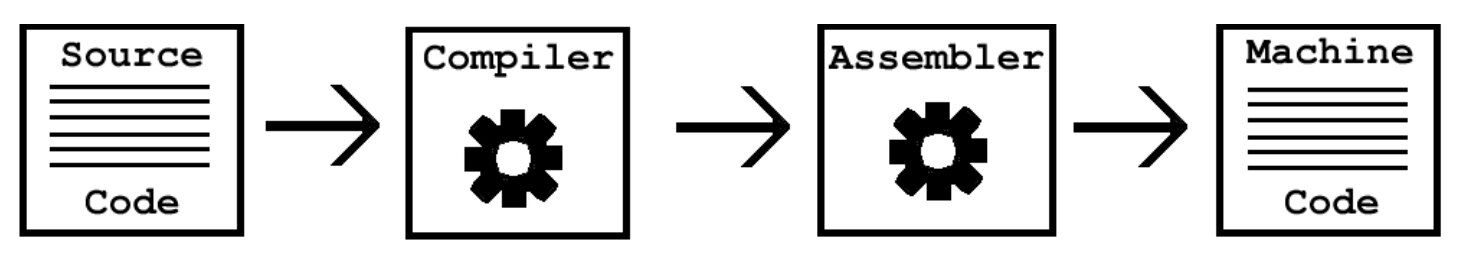
\includegraphics[width=.8\textwidth]{media/Source2Executable.jpg}
    \caption{Quellcode (engl. ``source code'') wird in ausführbaren Maschinencode umgewandelt \cite{stallman2002}}
\end{figure}

Hier als Beispiel der Source Code zu einem simplen Programm \textit{helloworld.c} geschrieben in der Programmiersprache C, welches in der Konsole ein simples \say{Hello World} ausgibt:

\lstset{language=C}
\begin{lstlisting}
#include <stdio.h>

int main() {
    printf("Hello World\n");
    return 0;
}
\end{lstlisting}
%TODO: idk mir sötte grundlegendi sache ned erkläre
Ein Teil der kompilierten, ausführbaren Version des Programmes \textit{./helloworld} sieht aber so aus:
\begin{lstlisting}
0011010001100000010111110110111101101100011001110110001001101111011011000110000101100100
1111101101111011101000111001101110010011000010101111100000000000000110100011100000111100
1101010110001100000000011011010110111101101100011100000111010001100101011001000110010100
0000010111001011111000000000000000000000011010010000000011001000101111101011111011011110
1100011001110110001001101111011011000110000101100100010111110110111101110100011100110111
0000000000000001101001001000001100001010111110111100001110101011001100101111101101110011
\end{lstlisting}

Wie man sieht, geht bei diesem Prozess des Kompilierens die Lesbarkeit für den Menschen grösstenteils verloren. Um ein Programm ausführen können braucht der Nutzer also keinen Zugang zum Quellcode. Doch wenn er wissen will, was das Programm macht - es könnte ihn ausspionieren oder andere bösartige Sachen im Hintergrund machen - oder einfach das Programm verändern will, braucht er unbedingt Zugang zum Source Code.\\

\subsubsection{Lizensierung}
% ENG: The differences of different source code models and their licenses have been already discussed in this paper (?). The reason the GNU General Public License Version 3 (short: GPL v3) was chosen because it is one of the most popular and strongest copyleft licenses that suits the application.
Grundsätzlich gibt es die  Unterscheidung zwischen freien Softwarelizenzen proprietären Softwarelizenzen. Doch auch bei Open Source Software gibt es verschiedene Lizenzmodelle welche gewählt werden können. Diese lassen sich ziemlich gut in zwei Kategorien unterteilen: in \gls{permissive} und in \gls{copyleft}.\\

Die Autoren dieser App halten Copyleft Software in ethischer und praktischer Hinsicht für die beste Wahl bei der Softwarelizensierung, wehalb entschieden wurde für dieses Softwareprojekt die \textit{GNU General Public License (GPL) Version 3} \cite{GPLv3} der \gls{fsf} zu verwenden, da diese eine der bekanntesten, strengsten und somit effektivsten Copyleft-Lizenzen ist.

\subsubsection{Philosophie (suckless)}

\begin{nicequote}{Many (open source) hackers are proud if they achieve large amounts of code, because they believe the more lines of code they've written, the more progress they have made. The more progress they have made, the more skilled they are. This is simply a delusion.}{https://suckless.org Manifest \cite{suckless}}
\end{nicequote}

% ENG: (Nowadays) a lot of Open Source Developers pride themselves in writing software with much features that cater to the non-technical enduser. This results in having a large codebase, which gets bigger and bigger with every release. This makes it harder to maintaining the ever growing codebase, more and more bugs occurs, security and (most importantly) performance struggles under these conditions. This degrades the quality of software technology as it is the mainstream narrative to ``save time and money''.\\

Eine grosse Anzahl Open-Source-Entwickler stolz darauf, Software mit scheinbar möglichst vielen Features zu schreiben. Dies führt zu einer großen Codebasis, die mit jedem Release größer und größer wird. Dadurch wird es schwieriger, die ständig wachsende Codebasis zu unterhalten, es treten immer mehr Fehler auf, die Sicherheit und - vor allem - die Leistung leidet unter diesen Bedingungen. Dies führt zu einer Verschlechterung der Code-Qualität der Software, da es die gängige Praxis ist, ``Zeit und Geld zu sparen''. \cite{bhattacharya2020}\\


% ENG: This is where the \textit{suckless philosophy} comes in place: It aims at making software with simplicity in mind: Less source lines of code to not render the project unmaintainable in similar way as mentioned above. This way of programming is a lot more difficult, but the struggle is most of the time worth it. This coding philosophy also incentives (quality) code rewrites - which happens a lot less with bloated software counterparts - that gives the user more alternatives to choose from.

Hier kommt die Philosophie des \textit{Suckless Philosphy} ins Spiel: Sie zielt darauf ab, Software mit Hinblick auf Einfachheit zu entwickeln: Weniger Quellcodezeilen, um das Projekt nicht in ähnlicher Weise unmaintainable zu machen, wie oben erwähnt. Diese Art zu programmieren ist viel schwieriger, aber der Aufwand ist es meistens wert. Diese Programmierphilosophie bietet auch Anreize für das qualitativ hochwertige Neuschreiben von Programmen - was bei der sogenannten \textit{Bloated Software \cite{bhattacharya2020}} viel seltener vorkommt - und gibt dem Benutzer mehr Alternativen zur Auswahl.

\paragraph{Hintergründe, Technologisch, UNIX, KISS}
Die \textit{Suckless Philosophie} ist aber längst nicht die erste Philosophie im Softwarebereich welche auf Simplizität beruht; so beispielsweise eine beliebte Definition der altbekannten \textit{UNIX Philosphy}:

\begin{nicequote}{This is the Unix philosophy. Write programs that do one thing and do it well. Write programs to work together. Write programs that handle text streams, because that is a universal interface.}{A Quarter Century Of UNIX \cite{salus1994}}
\end{nicequote}

Bekannt ist auch das \textit{KISS Prinzip}: \say{Keep it simple, stupid}. Dieses Prinzip kommt ursprünglich vom U.S. Admiral Stroop, der das \say{Project KISS} 1960 ins Leben gerufen hatte, welches die Verlässlichkeit verbessern und die Kosten für amerikanische Militärausrüstungen senken soll. \cite{dalzell2009} Gerne wird diese Prinzip zitiert, wenn jemand der Meining ist, unnötige Komplexität sei vorhanden in einem Softwareprojekt.


\begin{comment}
\section{Programmier-Tools}

\subsection{Hardware}



\subsubsection{Smartphones}
% ENG: We used different Models of Smartphones running different variants of the android operating system to install and test our app. It was also used to compare it and benchmark it against our competition (the already existing mail clients on android).

Es wurden verschiedene Smartphone Modelle genutzt um die App auf verschiedenen Androidversionen testen zu können. Sie wurden auch genutzt um unsere App mit der Konkurrenz zu vergleichen und die 
Konkurrenz zu begutachten. 

\subsubsection{PC / Laptop}
% ENG: The usage of computers was to the actual work of creating the software, documentation and the text of this paper (?).

Der Gebrauch von Computern wurden gemacht um die Software, die Dokumentation und dieses Maturschreiben zu erstellen. 
\subsection{Software}

Aufgrund dessen, dass ein umfassendes Programm entstehen soll, wird auch Gebrauch von einigen anderen Programmen, Bibliotheken und sonstigen Tools gemacht. In den nachfolgenden Seiten wird beschrieben welche Programme genutzt werden, wieso diese ausgewählt wurden und wie der Umgang mit ihnen war.  


\subsubsection{Programme}

\paragraph{Version Control System}

% ENG: For developing software above a certain level of complexity, it helps to use a so called VCS (Version Control System). This is a software/system that manages the versioning of software. This is useful so you don't have to for example create MANUALLY a new folder for every new version and copy the code with the new changes in there. This would be not very user friendly, wasteful of disk space and overall very inefficient. These systems also make it easy to synchronise projects to a remote server to allow for easy collaboration on multiple devices and for different developers.\\
Für die Entwicklung von Software ab einer gewissen Komplexität ist es hilfreich, ein so genanntes VCS (Version Control System) zu verwenden. Dabei handelt es sich um eine Software/System, das die Versionierung von Software verwaltet. Das ist nützlich, damit man nicht für jede neue Version manuell einen neuen Ordner anlegen und den Code mit den neuen Änderungen dorthin kopieren muss. Das wäre nicht sehr benutzerfreundlich, würde Speicherplatz verschwenden und wäre insgesamt sehr ineffizient. Diese Systeme erleichtern meist auch die Synchronisierung von Projekten mit einem Webserver, um eine einfache Zusammenarbeit auf mehreren Geräten und für verschiedene Entwickler zu ermöglichen.\\


\subparagraph{Git}
% ENG: It also allow for additional advanced features like branching a repository, which means developing multiple features separately from each other to then later merge the changes together, when each of the features are working as expected.
Git ist das für dieses Projekt verwendete VCS. Es ist das meistverbreitete Tool unter Softwareentwicklern und dabei ermöglicht auch zusätzliche fortgeschrittene Funktionen wie das \textit{Branching} eines Repositorys, was bedeutet, dass mehrere Funktionen getrennt voneinander entwickelt werden, um dann später die Änderungen zusammenzuführen, wenn jede der Funktionen wie erwartet funktioniert. So etwas sieht der \textit{Git Flow} generell und auch in diesem Projekt aus:

\begin{figure}[H]
    \centering
    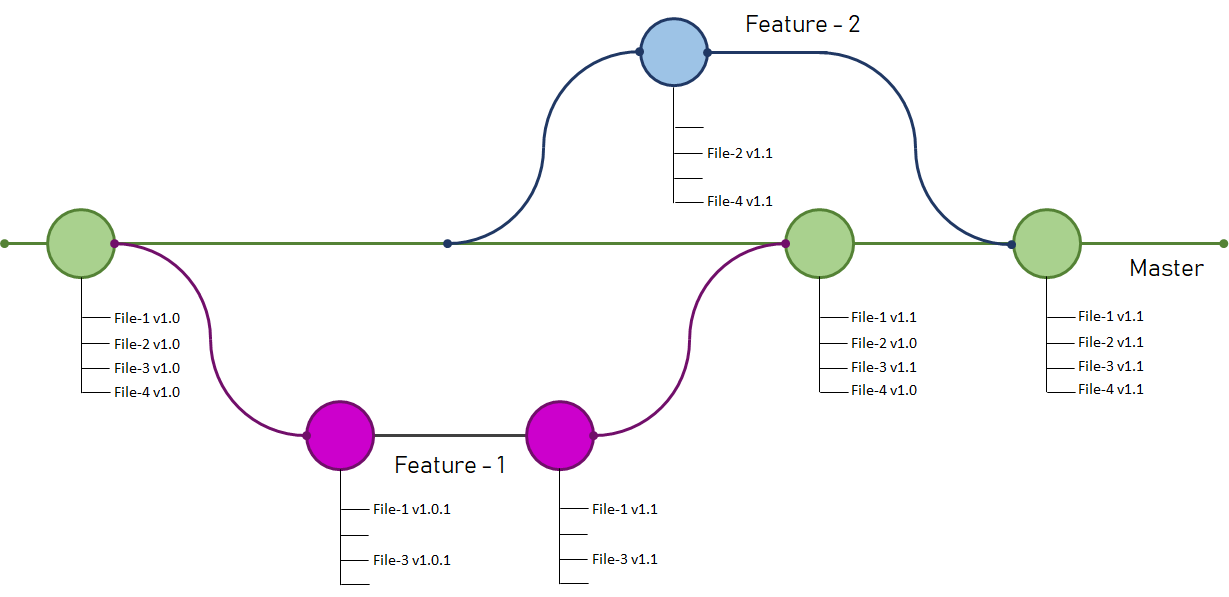
\includegraphics[width=.8\textwidth]{media/gitflow.png}
    \caption{parallele Featureentwicklung mit Git \cite{gitflowBlog}}
\end{figure}

\subparagraph{Github}

% ENG: This is our remote git server. But is is more than just a git server, it is a popular platform with over 50 million (software) repositories that people search to find interesting software. So we can use this to make our software more searched and popular (but this is not considered of great importance).
Das ist der hier verwendete Git Server. Aber eigentlich es mehr als nur ein einfacher Git-Server, denn es ist auch eine populäre Plattform mit über 238 Millionen Software Repos (Stand September 2021 \cite{githubRepoQuery}) welche gerne durchsucht werden, um interessante Software zu finden. Das kann also benutzt werden dieses Softwareprojekt berühmter zu machen, was aber nicht von hoher Wichtigkeit erachtet wird.


\paragraph{IDE}
 % eng IDE stands for ``Integrated Development Environment''. This means a program where the coder edits, debugs the code. It provides more features than just editing text, but also advanced autocompletion features and warnings/suggestions that the programmer should do something differently because of various reasons of bad programming practice. These programs have a lot of great features, but are often buggy, resource hungry and slow, like our choice of IDE: Android Studio.
IDE steht für ``Integrated Development Environment''. In diesem Programm editiert und debuggt der Programmiere seinen Code. Solche Software verfügt dabei um mehr Features als nur Texteditierung, sonden auch nützliche Autocompletion Features und gibt Warnungen oder Vorschläge, was der Programmier besser machen sollte. Solche Programme haben zwar viele nützliche Features, wovon wir nur einen Bruchteil kennen oder brauchen, sind aber oft buggy, resourcenhungrig und langsam. So auch die IDE Wahl dieses Projekts: Android Studio. Diese IDE wurde auch gewählt da sie stark optimiert und extra für die Androidentwicklung gemacht wurde.

% \paragraph{Texteditor}
% Text editors to have less ``advanced'' coding-related features, so they are not optimal for big projects with lots of files and graphical content.

\paragraph{Android Emulator}
% ENG: An emulator is a program that simulates an device/operating system so that you can run inside another operation system. We use an Android Emulator inside of our GNU/Linux running on our computer, so that we do can test our app without always having to transfer it to an actual phone running android natively.

Ein Emulator ist ein Programm, welches ein Gerät oder Betriebssystem simuliert, sodass man es innerhalb eines anderen Betriebssystems laufen lassen kann. Für dieses Projekt wurde von Android Emulatoren Gebrauch gemacht, um die App gleich auf dem Computer testen zu können, wo man gerade am programmieren ist. So muss nicht ständig die App auf ein Smartphone transferiert werden, wo Android nativ läuft, nur um die App austesten zu können.

\paragraph{Compiler}
Um die \say{.apk}-Datei zu kompilieren, benutzen wir ein \textit{Build Automation Tool designed for multi-language programs} namens Gradle. Dieses Programm erleichtert den compile Prozess, da der Kompilationsprozess recht komplex wäre, wenn man ihn manuell machen würde. Man müsste alle Dependencies selber angeben, herunterladen und Up-to-Date halten. Durch die Verwendung solche Build-Automatisierungstools sparen wir zwar an Arbeit, und auch viel kürzer wäre das kompilieren ohne Gradle auch nicht.

\paragraph{Installer / Packaging}
% ENG: When we compiled our app using gradle, we get an .apk file as its output. APK stands for Android Package, which is the Package Format used for installing most of the software in Android. However, there are to sorts of apk that are compiled: a debug apk and a release apk. The debug version has extra features compiled in that help auditing bugs and new features not ready for using in the app available to users. The release Version has the current version number (?) added to it and is what you need to distribute of your working version to your users.
Nachdem die App mit \textit{Gradle} kompiliert wurde, erhält man eine .apk-Datei als Output. APK steht für Android Package, was das Packaging Format ist um Software zu installieren auf Android. Dabei kann man die App aber auf zwei Arten kompilieren: eine \textit{debug APK} oder eine \textit{release APK}. Die Debug Version bekommt extra Features hinein kompiliert welche dem Entwickler helfen Bugs zu finden und zu prüfen. Diese Version wird verwendet um neue Features auszutesten, welche noch nicht bereit sind für die Nutzer. Die Release Version enthält die derzeitige Versionsnummer und ist das was man braucht, um eine funktionierende Version der App den Nutzern zur Verfügung zu stellen.

\subparagraph{signing keys}
% ENG: Nearly all Android Systems are configured to only allow application that are signed with a key from the developers. This is done for various reasons like security, compatibility checks and other . So before we can install our app on 99\% of Smartphones, we first have to sign it with our cryptographic key we have created. Of course, this is only needed for actual releases and not for using debugging version e.g. in your android emulator.
Fast alle Android-Systeme sind so konfiguriert, dass sie nur Anwendungen zulassen, die mit einem Schlüssel des Entwicklers signiert sind. Die Argumentation, weshalb das bei Android benötigt wird ist Sicherheit: Durch das Kryptographische signieren von Apps werden potenziell schädliche Modifikationen nach Kompilation der App erschwert. Dieses Verhalten stört die meisten Appentwickler nicht und ist sogar eher erwünscht.\\

Bevor wir also unsere App auf 99\% der Smartphones installieren können, müssen wir sie zunächst mit einem kryptografischen Schlüssel signieren, der von den Entwicklern dieser App erstellt wurde. Dies ist natürlich nur für die tatsächliche Veröffentlichung erforderlich und nicht für die Verwendung der Debugging-Version, z.B. in einem Android-Emulator.

\subparagraph{Android Debugging Bridge}
% ENG: This is a software tool to interact with android devices that are connected to a computer via usb. With it you can do useful thinks like screenshots, screen recordings, transferring files to and from your computer and installing / removing packages.

Dies ist ein Software-Tool für die Interaktion mit Android-Geräten, die per USB mit dem Computer verbunden sind. Damit kann man nützliche Sachen wie Screenshots, Bildschirmaufnahmen, das Übertragen von Dateien und die (De-) Installation von Apps, resp. Softwarepaketen.

\paragraph{Open Source Programme}

Beim Programmieren kann es sehr hilfreich sein Programme zu haben welche, ähnliche Funktionen haben wie das Programm welches entstehen soll. 
Solche Vorlagen können beliebig getestet und verändert werden. Simon hatte zu Beginn Schwierigkeiten Java zu nutzen, um Programme zu schreiben, da er noch nicht viel 
Erfahrung mit dem Programmieren hatte. Um sich mit der Art der Sprache und des Programmierens vertieft auseinander zu setzen, begann er Email-Apps, welche Open Source
waren, genauer zu Betrachten. Zu beginn haben diese Programme grosse Teile des Programms ausgemacht doch gegen Ende wurde sie so oft überarbeitet, dass es
kaum noch eins zu eins Ausschnitte aus diesen Programmen gibt. \\

Als Basisprogramm für die Roomdatabase hat Simon ein Open source Programm gebraucht, welches als Tutorial diente. \cite{roomApp}

Stark davon betroffen sind die Dateien EmailViewModel.java, EmailViewHolder.java, CustomAdapter.java, EmailRepository.java, EmailRoomDatabase.java, Message.java, MessageDao.java
und NewDraftMessageActivity.java. Bei diesen
Dateien handelt es sich um fast Kopien des Basisprogramms, sie wurden stark erweitert und sie werden von anderen Funktionen aufgerufen. 
Die Dateien ArchiveFragment.java, GalleryFragment.java, HomeFragment.java, DraftFragment.java, SpamFragment.java und MainActivity.java beinhalten alle fünf Zeilen beginnend mit der 
Variabel mEmailViewModel vom Typ EmailViewModel. Diese fünf Zeilen sind jeweils auch aus dem Basisprogramm. 
Weiter beinhaltet die Datei MainActivity.java eine Funktion namens onActivityResult von Zeile 183-215, welche auch aus dem Basisprogramm stammen. 
Sehr ähnliche Zeilen befinden sich auch in der messageCreateFragment.java Datei von Zeile 120-140. Diese Stammen ursprünglich auch aus dem Basisprogramm, wurden aber natürlich bearbeitet. \\





% \subsubsection{Librarys}
% (bedeutung im glossar erklärt)

\subsection{Recherche Tools / Quellen}
\subsubsection{Internet}
% ENG: In the world wide web we use search engines like DDG (duckduckgo.com), the Arch Linux Wiki, Wikipedia and more programming-related websites like SOV (stackoverlow.com).
Um das Netz besser durchsuchen zu können, wurden Suchmaschinen wie DDG (duckduckgo.com), das Arch Linux Wiki, Wikipedia und programmierbezogene Internetseiten wie SOV (stackoverflow.com);
\subsubsection{Bücher, Artikel}
% ENG: We used different books and articles physically and digitally sometimes for the programming/coding process, but mostly for the text of this paper.
Es wurde auch Nutzen gemacht von Büchern und Artikeln, in digitaler und physischer Form, ein wenig für den Programmierprozess, aber hauptsächlich für den Maturarbeitstext.

\subsection{Dokumentation(-stools)}
\subsubsection{Latex}
% ENG: To write more formatting-demanding papers like in this paper it was made use of the typesetting engine LaTeX. This is a highly extensible and efficient way for getting your paper to look just like you want it.
Um formatierungsintensivere Texte wie diese Arbeit zu schreiben, wurde das Satzprogramm LaTeX verwendet. Dies ist ein äußerst erweiterbarer und effizienter Weg, um eine Arbeit so aussehen zu lassen, wie man es exakt verlangt. Es wird nicht umsonst extensiv verwendet in naturwissenschaftlichen Artikeln, Büchern und Verlagen.
\subsubsection{Pandoc}
% ENG: This is program to convert from one document format to another. This is useful to write a document in format with very simple syntax (e.g. markdown) to convert it to a format that allows much better formatting (e.g. LaTeX) without having to use the more sophisticated syntax of the latter format. This is often used to write documentation or short texts with the minimal amount of time and effort to do so.
Dies ist ein Programm zur Konvertierung von einem Dokumentformat in ein anderes. Dies ist nützlich, um ein Dokument in einem Format mit sehr einfacher Syntax (z.B. Markdown) zu schreiben und es in ein Format zu konvertieren, welches eine viel bessere Formatierung ermöglicht (z.B. LaTeX), ohne die anspruchsvollere Syntax des komplexeren Formats verwenden zu müssen. Dies wird häufig verwendet, um Dokumentationen oder kurze Texte mit minimalem Zeit- und Arbeitsaufwand zu schreiben. So auch bei dieser Arbeit.

\end{comment}

\subsection{Arbeitsziele}

Wir wissen, was ein Email Client können muss, und haben nicht vor eine App zu designen, welche vollkommen überladen ist, mit Funktionen die keiner braucht.\\

Die App soll die Basisfunktionen eines klassischen Email-Clients erfüllen. Dazu gehören das Lesen, Schreiben, Empfangen und Versenden von Emails, 
das Öffnen und Anfügen von Anlagen, die Setzung einer Email-Signatur und das Erstellen und Speichern von Entwürfen. 
Ebenso soll es verschiedene Ordner unterstützen, wie z.B. ein Spam/Junk oder ein Archiv Ordner. 
Dazu soll es möglich sein E-Mails visuell sortieren zu können, beispielsweise indem die Ordner im Client nach Datum des Empfangs oder dem Absender sortiert werden können. E-Mails sollen markiert, gelöscht und weitergeleitet werden können und es soll eine Suchfunktion für jeden Mailordner geben. \\

Ebenso soll es einen Account Manager geben, was voraus setzt, dass es möglich ist sich mit verschiedenen 
Accounts anzumelden und diese bei bedarf zu wechseln. Beim Anmelden einer E-Mail, soll es dem Nutzer leicht gemacht werden, mit eingebauten Konfigurationen für beliebte 
Emailprovider in der Schweiz. Darunter diese Anbieter: stud.edubs.ch, gmail.com, gmx.ch, outlook.com, yahoo.com, icloud.com, hotmail.com, web.de. \\

Ein Element, welches fast jede App Heutzutage hat, sind Pushnachrichten, welche auch eingebaut werden sollen. Dabei sollen neue Nachrichten mit dem Absender und dem Beginn der E-Mail angezeigt werden. 
Dies soll ein weiteres Feature der App sein. Wie es für leichte Email-Clients oft üblich ist, werden Bilder erst angezeigt, sobald es der Nutzer ausdrücklich möchte. Dieses Verhalten soll in den App-Einstellungen steuerbar gemacht werden. Eine sehr praktische Funktion soll sein, dass E-Mail-Adressen gespeichert werden und beim schreiben einer neuen E-Mail direkt verfügbar sind und ausgewählt werden können. Ob diese Funktion sinnvoll ist, ist fraglich, da auf viele Leute keine Emailaddressen auf der Kontaktapp ihres Handys speichern.\\

Das letzte Feature soll sein, dass Links direkt in einem Browser geöffnet werden können. Die Einstellungen sollen zudem das Farblayout der App ändern können, die Synchronisationsintervalle ändern können, Einstellungen an den Pushnachrichten ändern können, Kontaktlisten verwalten und Einstellungen zu Privatsphäre beinhalten.


Im Unterschied zur Konkurrenz soll diese App so programmiert werden, dass sie alle nötigen Grundfunktionen für einen Email Client auf dem Smartphone beinhaltet, aber schneller starten soll als die Apps der Konkurrenz, weniger Speicherplatz und Resourcen verbrauchen soll und nicht mit unnötigen Funktionen überladen sein. \\


Ein Pluginmanager soll auch eingebaut werden, um weitere Funktionen, welche das Programm verlangsamen würden oder nicht für jedermann geeignet sind, hinzuzufügen können. Es existiert natürlich auch die Möglichkeit nach Abschluss dieser Arbeit die App zu verbessern und auf uns an Nutzerwünsche anzupassen, doch hier wurden jetzt die ungefähren, geplanten Grundfunktionen genannt, um die Ziele der Funkionalität besser zu beleuchten.\\
Wir haben uns viele Ziele gesetzt und dachten, dass wir auch mehr schaffen können. Weshalb dies nicht der Fall ist wird noch genauer betrachtet. 




\section{Arbeitsprozess}

\subsection{Programmiermittel}

Um ein Programm, mir grösserem Umfang, zu Entwickel, braucht es Hilfsmittel die sich auf genau das spezialisiert haben. 
Eines dieser Hilfsmittel sind \gls{vcs}. Diese sind eine sehr praktische Methode um Funktionen in ein Programm einzubauen, ohne das Risiko 
das Programm komplett zu Überarbeiten, wenn diese Funktion einen Fehler hervorruft. In diesem Fall wurde \Gls{git} als \Glspl{vcs} genutzt, um für jegliche Funktionen
einen eigenen \gls{branch} zu erstellen und diesen wieder mit dem Hauptbranch zu \glspl{merge}, wenn die Funktion fertig ist.\cite{git} \cite{github} \\

Um zu Zweit an einem Projekt gleichzeitig zu arbeiten, gibt es viel Möglichkeiten sich das aktualisierte Projekt zur Verfügung zu stellen. Die einfachste ist sich das 
Projekt immer wieder zu Mailen, wobei schon nur bei Textarbeiten dabei Probleme auftauchen können, weshalb bei diesem Projekt \Gls{github} 
verwendet wurde. Über \gls{github} konnten die einzelnen Versionen des Programms, welche durch den Gebrauch von \gls{git} entstanden sind, geteilt werden. 
Auf \gls{github} ist das Programm öffentlich und wird dadurch auch open-source. Es kann aber nicht durch eine dritte Person, ohne Einwilligung von Noah, in den Source-Code
des Programms geschrieben werden. Falls dies aber der Fall gewesen wäre, würde die dritte Person als mitwirkende Person auf \gls{github} aufgelistet werden. \cite{github} \\

Beim Programmieren einer grösseren Arbeit erweist es sich besonders nützlich ein \glspl{ide} zu verwenden. Es ist zu \gls{android-studio} gegriffen worden, weil sich dieses \gls{ide}
speziell auf die android Entwicklung spezialisiert hat. \gls{android-studio} besitzt viele Hilfsmittel, welche das Programmieren einer Androidapp erleichtert. Zum beispiel ist der
"Visual Layout Editor"\ eine grosse Hilfe beim Designen. \gls{android-studio} bringt auch einen \gls{compiler} und einen \gls{emulator} mit sich, womit eine \textit{debug} \gls{apk} und eine
\textit{release} \gls{apk} version der App erstellt werden kann. Um die App zu testen, wurde öfters ein \textit{debug} \gls{apk} File erstellt und auf dem \gls{emulator} aus \gls{android-studio}
getestet. Mit \gls{android-studio} können auch Apps mit speziellen Keys unterzeichnet werden, damit sie im GooglePlayStore veröffentlicht werden können.
Die App sollte aber nicht nur auf Emulatoren laufen, um auch das Gefühl des Designs besser zu empfinden oder den Gebrauch im Alltag zu testen, wurde eine \gls{adb} genutzt.
Mit \gls{android-studio} können auch Daten über die Effizienz der App aufgenommen werden. 
\cite{android-studio} \\

Open-Source Programme wurden bei dieser Arbeit öfters genutzt, um gewisse Funktionen einzubauen und ein Gefühl für das Programmieren solcher Funktionen zu bekommen. Die Programme
waren sehr 
hilfreich beim Lernen, da wir teilweise noch gar keine Erfahrung in gewissen Bereichen hatten. Was genau aus diesen Programmen entnommen wurde und um welche Programme es sich handelt, wird 
genauer im Anhang besprochen. 



\subsection{Programmstruktur}


\begin{comment}
\subsubsection{Sicherheit / Security (Features)}
% ENG: Considering that on 99\% of consumer smartphones the users do not even have root access (but which the ``owner'' of the smartphone software do have), people that are concerned with privacy or security would not use their important mailboxes on their smartphone anyway, but rather on their better secured computer running a Free Software Operating System etc.\\
In Anbetracht der Tatsache, dass auf 99\% der Consumer-Smartphones die Benutzer nicht einmal Root-Zugriff haben (den aber der ``Besitzer'' der Smartphone-Software hat), würden Leute, die auf Privatsphäre oder Sicherheit bedacht sind, ihre wichtigen Mailboxen ohnehin nicht auf ihrem Smartphone benutzen, sondern eher auf ihrem besser gesicherten Computer, auf dem ein reines Freies-Software-Betriebssystem läuft usw.\\

% ENG: Also taking in mind that the email protocol was written in a time with a still very limited access to computers, privacy and security where not in mind of its creators at the time is quite understandable. Why it still lasted to this day in this state is compromised on one side by networking effects and on the other side that simply most people neither know to technical detail nor care.\\
wenn man bedenkt, dass das E-Mail-Protokoll in einer Zeit geschrieben wurde, in der der Zugang zu Computern noch sehr eingeschränkt war und Datenschutz und Sicherheit nicht im Sinne seiner Schöpfer waren, ist das durchaus verständlich. Warum es sich bis heute in diesem Zustand gehalten hat, liegt zum einen an den \textit{Networking Effects} und zum anderen daran, dass die meisten Menschen die technischen Details einfach nicht kennen und/oder sich nicht darum kümmern.\\


% ENG: Nowadays it is possible to encrypt to content (body) of an email, but not the metadata, here the specification of the email protocol is to blame. This and just the fact that is was not BUILT as a secure or private way of messaging, makes emails not useful for these kinds of conversation. If you want to send your friends new plans on overtaking the world and establishing a global catholic monarchy without wanting anyone to know, your are a fool if you use email for that(granted, this is an over exaggerated example, but I hope the idea is clear).\\
Heutzutage ist es möglich, den Inhalt (Text) einer E-Mail zu verschlüsseln, nicht aber die Metadaten; hier ist die Spezifikation des E-Mail-Protokolls schuld. Dies und die Tatsache, dass es nicht als sichere oder private Art der Nachrichtenübermittlung konzipiert wurde, macht E-Mails für diese Art von Konversation unbrauchbar. Wenn Sie Ihren Freunden neue Pläne für die Übernahme der Welt und die Errichtung einer globalen katholischen Monarchie schicken wollen, ohne dass jemand davon erfährt, sind Sie ein Narr, wenn Sie dafür E-Mails verwenden (zugegeben, das ist ein übertriebenes Beispiel, aber ich hoffe, der Gedanke ist klar).\\

% ENG: So the conclusion for our application project is to not bloat up our app with hard-to-use security functions that just bloat the app and codebase unnecessarily. However we use sane security-focused default now further explained.
Die Schlussfolgerung für unser Anwendungsprojekt ist also, unsere Anwendung nicht mit schwer zu verwendenden Sicherheitsfunktionen aufzublähen, die die Anwendung und die Codebasis nur unnötig aufblähen. Es sollten jedoch vernünftige, auf Sicherheit ausgerichtete Standardeinstellungen genutzt werden, die u.a. jetzt näher erläutert werden.

%\subsubsection{PRIVATE MODE, Sandbox}
% ENG: When storing user settings (and data?), you can choose between different permission modes in android. We choose PRIVATE MODE, which means that apps with user permissions  can not see its content. But Google, root users, and apps with root access can easily bypass this restriction of the android permission system.\\
%Wenn man Nutzereinstellungen- und Daten speichert in Android, kann der Entwickler zwischen verschieden Berechtigungsmodi wählen. In diesem Project wurde der sogenannte \textit{PRIVATE MODE} gewählt. Dieser bewirkt, dass andere Apps mit Nutzerberechtigungen (also a alle von einem Nutzer installierten Apps) den Inhalt dieser Daten nicht sehen können. Aber Google, Root-Nutzer und Apps mit Root-Zugriff können diese Einschränkung des \textit{Android Permission Systems} ohne weitere Probleme umgehen.\\

\subsubsection{Code Kompaktheit}
% ENG: This is something that we have absolutely achieved, we used so much less SLOC than any of the competing email clients on android.(compare use of libraries, and if we used more or less than the other apps) This is also very crucial to stand with our initial goal and the suckless philosophy. While we used \~ 4000 SLOC, other apps use a whopping 300'000 SLOC.
Das ist etwas, was im Laufe diese Projekts ziemlich gut eingehalten wurde: Es wurden viel weniger SLOC geschrieben als bei den konkurrierenden Email Clients auf Android. Das ist ein sehr wichtiger Massstab um das initiale Ziel der \textit{Suckless Philosophy} so gut wie möglich zu erreichen. Während dieses Projekt nur \~ 4000 SLOC Zeilen Code aufzuweisen hat, sind es bei anderen Apps gar über 300'000 SLOC.
\subsubsection{Maintaining}
% ENG: Our codebase should be very easy to maintain: The main things you would have to do is check if the dependencies are up to date and if they can be considered deprecated.\\
Die Codebasis dieses Projektes sollte sehr einfach zu maintainen sein: Die wichtigsten Punkte dabei sind, dass der Maintainer schaut, dass die Dependencies auf der neusten Version sind und ob sie als obsolet oder veraltet angesehen werden müssten.\\

% ENG: Even if this project gets abandoned by their original developers - or as some people call that: when it get orphaned - and if someone finds it and likes it, he can easily read through it and understand the code without too much effort needed of understanding the codebase. Would the same be the case for bloated programs like thunderbird? I don't think so either.
% TODO: get source to term 'orphaned packages'
Selbst wenn das Projekt aufgegeben werden sollte bei seinen ursprünglichen Entwicklern und jemand das Projekt findet und es ihm gefällt kann er dann recht einfach und schnell die Codebase durchlesen und sie ohne allzu grossen Aufwand verstehen. Wäre das auch der Fall bei bloated Software wie thunderbird? Das glaube ich auch nicht.

\subsubsection{less bug/error-prone}
% ENG: This is thanks to the suckless nature of our coding philosophy, but also our execution. It could be the case however that bad practices may have been used as the initial project owner did not have a lot of experience of 
Es ist grösstenteils der suckless-basierten Codingphilosophie zu verdanken, aber auch der Umsetzung. Es könnte jedoch der Fall sein, dass schlechte \textit{Coding Practices} verwendet wurden, da die beiden initialen Entwickler dieses Projekts nur eine beschränkte Erfahrung mit der Androidentwicklung mit der Java-Programmiersprache hatten.
\end{comment}


%\subsection{Informationsbeschaffung}
% TODO: in den rest des texts integrieren

%Zu beginn der Arbeit konnten Noah und Simon noch kein Java. Noah kannte sich gut aus mit Programmiersprachen und konnte es deshalb mit Java ruhig angehen.
%Simon hingegen wusste, dass er noch viel zu lernen hatte. Er erhoffte sich die Grundlagen im Informatik Unterricht zu lernen. 
%Simon lernte auch einige dinge, jedoch ging ihm das zu langsam und er schaute sich nach anderen Lernmöglichkeiten um. 
%Zu diesem Zeitpunkt konnten einige Schüler an einem Programm mitmachen, bei welchem sie in die Uni gingen und gewisse 
%Vorlesungen besuchen konnten. Ein Klassenkamerad von Simon konnte von diesem Programm profitieren und besuchte Informatik. 
%Dort lernte er in einem unglaublichen Tempo Java, weshalb Simon seinen Klassenkameraden fragte ob er seine Unterlagen ausleihen konnte. 
%Sein Klassenkamerad war so freundlich und übermittelte ihm die Unterlagen. So konnte Simon auf effektive weise Java lernen. \\
%
%Persönlich hatte Noah schon Erfahrung mit verschieden Programmiersprachen. Am ähnlichsten zu Java waren dabei meiner Einschätzung nach C und C++, welche eine teilweise ähnliche Sytax gegenüber Java aufweisen. Wirklich etwas mit Java gemacht hat er bei der Pluginprogrammierung für Minecraft und im EF (Ergänzungsfach Informatik) am GKG (Gymnasium Kirschgarten).\\
%
%Als nächstes ging es darum wie eine App aufgebaut ist und wie zwei Personen Zweitgleich an einem 
%Programm arbeiten konnten. Dafür musste sich Simon über Git/Github informieren. Noah hatte ihm ein Video empfohlen, welches 
%Simon studieren soll und er soll kleine Übungen mit Git ausprobieren um ein Gefühl dafür zu bekommen. Die beiden Informierten 
%sich über verschiedene Plattformen wie eine App funktioniert und wie sie aufgebaut ist. \\ 
%
%Es ging langsam voran und die beiden begannen mit technischen Einstellungen. Als erstes 
%wurde Android Studio  und eine ADB installiert. Noah hat sogar eine Anleitung zur Installation von ADB geschrieben. 
%Um diese auszuprobieren und die Grundlage zu schaffen auf welcher Simon und Noah die nächsten paar Monaten arbeiten werden, haben sie ein
%Testprogramm erstellt namens "Hello World". Es war ein ganz simples Programm das nur zum Testen der Infrastruktur diente. 
%Sie haben ein Gradle.build file erstellt, dies dauerte erstaunlich lange. Später erkannten sie das diese Verhalten sehr üblich für 
%Gradle ist. Nach einiger Zeit haben es beide geschafft ein apk file zu besitzen, welches erfolgreich die "Hello World" app beinhaltete und ausführt. 
%Anschliessend erstellte Noah ein GitHub repository in welchem die beiden das Programm teilen werden. \\

% \textbf{ https://www.youtube.com/watch?v=2sjqTHE0zok} nur um später zu makieren.

\subsubsection{Hauptziele}
Gemäss den Zielen soll die App eine Verbindung mit einem Server erstellen können und mit ihm Interagieren können. Heisst sie soll die Informationen über einen Account, die der 
Nutzer eingibt überprüfen können und weiter die Emails die ein Nutzer auf einem \gls{server} hat herunterladen. Ebenso soll die App Nachrichten weiter über einen Server verschicken können. 
Um das zu realisieren, haben sich die Autoren nach passenden \glspl{library} für Java umgeschaut. Das Resultat dieser Suche waren zwei Libraries. 
%TODO: noah schrib wurum mir die libraries ned gange sind und wurum mir uf python umgstiege sind. 

Weil nach dem herunterladen der Nachrichten vom Server viele Daten gespeichert werden müssen, muss eine Möglichkeit her, wie diese Daten möglichst schnell, 
und der Einfachheit halber mit einer gewissen Abstraktion, in einer sinnvollen Datenstruktur gespeichert werden können. Dazu taugte eine \gls{database}. Um dies zu erreichen 
liest sich einer der Autoren in ein Buch ein. Dieses Buch soll ihm Aufschluss über das erstellen einer Database geben. 
Es wurde klar, dass eine Database für Android meist mit \gls{sql} oder \gls{sqlite} geschrieben wird. Jedoch sind diese Sprachen nicht wirklich handlich und es
liess sich auch nicht mit dem Zeitplan verknüpfen eine weitere Programmiersprache zu lernen. Weshalb zu Room gegriffen wurde. Room ist eine abstrakte Klasse über SQLite 
und kann mit dieser Kommunizieren. Mit ihr können SQL \glspl{query} fast vollständig in Java geschrieben und ausgeführt werden. Ebenso ist Room für die Fehlersucher besser geeignet, 
weil es beim Compilen der App die SQL queries und \glspl{entity} überprüft. \cite{roomInfo} \\

Um die heruntergeladenen und gespeicherten Nachrichten auch Anzeigen zu könne wird ein Interface benötigt. Dieses sollte so schlicht und ordentlich wie möglich gehalten werden. 
Die \gls{recyclerview} Library ist eine optimale Möglichkeit Daten in Form von Nachrichten als eine Auflistung zu zeigen. Sie bringt einen Vorteil gegenüber einer \gls{list} mit und zwar
verwendet sie \glspl{view}, die Angezeigt wurden, wieder. Was dem Recyclerviewer einen Vorteil im Punkt Effizienz gegenüber der Liste bringt. \cite{recyclerViewRecycle}

Neben der Recyclerview Library werden auch andere libraries gebraucht um das \gls{user interface} zu erstellen. Einer dieser libraries ist Material oder Material Design. 
Den Autoren hat sie schlicht gefallen und sie ist nicht schwer zu benutzen, weshalb diese Library genutzt wurde. Sie ist nach ganz klaren Prinzipien aufgebaut 
und von Google erstellt worden um hochwertige Designs zu kreieren. \cite{materialDesigne}


\subsubsection{Aufbau}

Die App kann grob in drei Teile unterteil werden. In \textit{User Interface}, in \textit{Database} und in \textit{Serververbindung}. 

\begingroup
\setlength{\intextsep}{7pt}
\setlength{\columnsep}{15pt}

\begin{wrapfigure}{r}{10cm}
\centering
    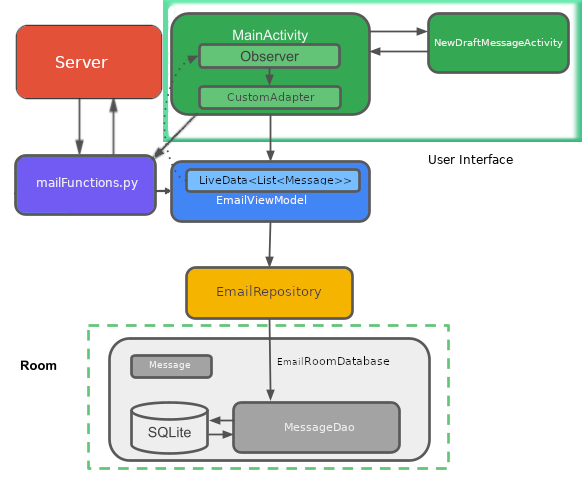
\includegraphics[scale=.52]{media/AppStructureFull.png}
\caption{Grob Aufbau der App}
\end{wrapfigure}

\nohyphenation

Diese drei Komponenten bilden zusammen die App, wobei der Teil der Serververbindung nicht immer aktiv ist. Er wird von dem User Interface
aufgerufen, wenn zum Beispiel sich ein neuer Nutzer mit einem Emailaccount anmelden möchte. Dann werden die Accountdaten an de Server geschickt und überprüft.
Wenn diese korrekt sind werden alle Nachrichten, die dieser Nutzer auf dem Server hat, heruntergeladen und weiter an die Database gegeben. Abgesehen von dem 
Speichern der Nachrichten die frisch vom Server kommen, macht die Database nur noch zwei dinge. Sie kann, durch das Interface entstandene, Nachrichten so abspeichern, dass sie 
vom \textit{User Interface} im Ordner \textit{Draft} angezeigt werden. Und die \textit{Database} kann weiter gespeicherte Nachrichten bearbeiten so, dass sie vom 
\textit{User Interface} in eine anderen Ordner angezeigt werden.

\endgroup

\newpage
\subsubsection{Startup UI}


%I then made the app more functional, so that you have a base GUI with a drawer, a menu in the bottom and in the drawer navigation menu you can tap on the «Add Email» Button and a popup window will come up asking you for name, email and password. Even the save and cancel button work. Now we only need a functionality to save this information to a string somewhere in the main activity.\\

\begin{figure}[H]
\centering
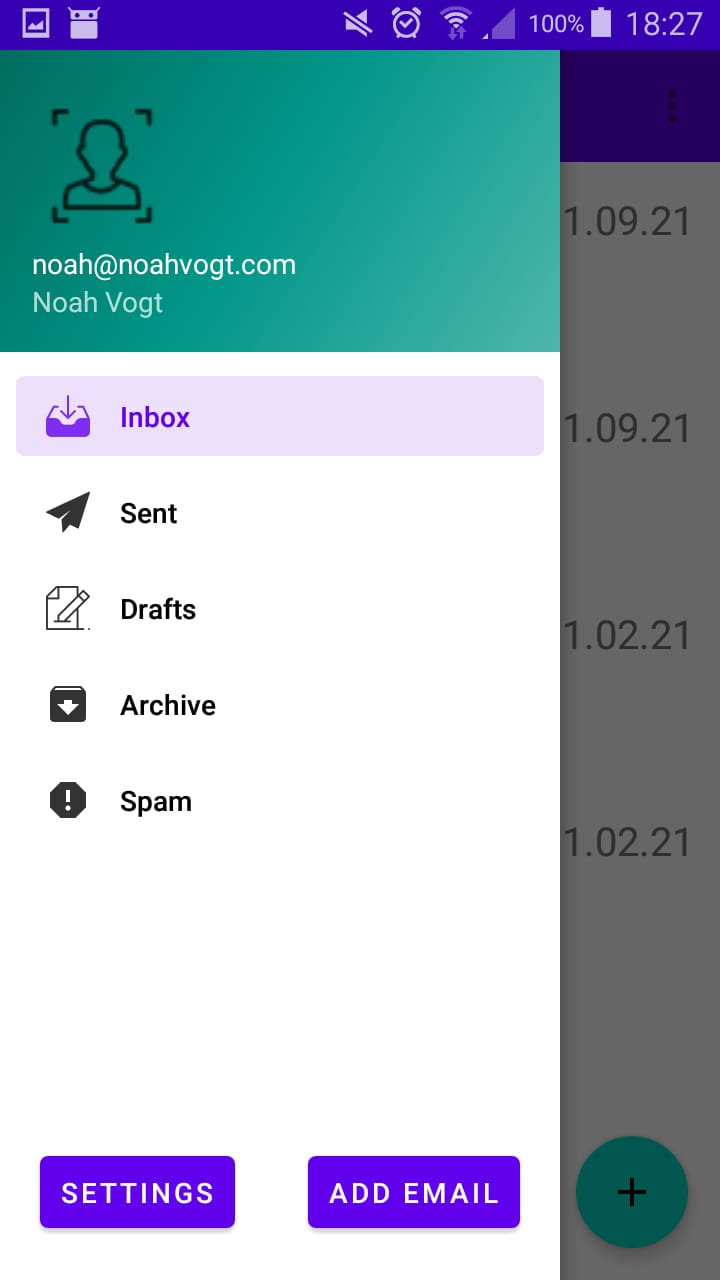
\includegraphics[width=.32\textwidth]{media/drawer.jpeg}
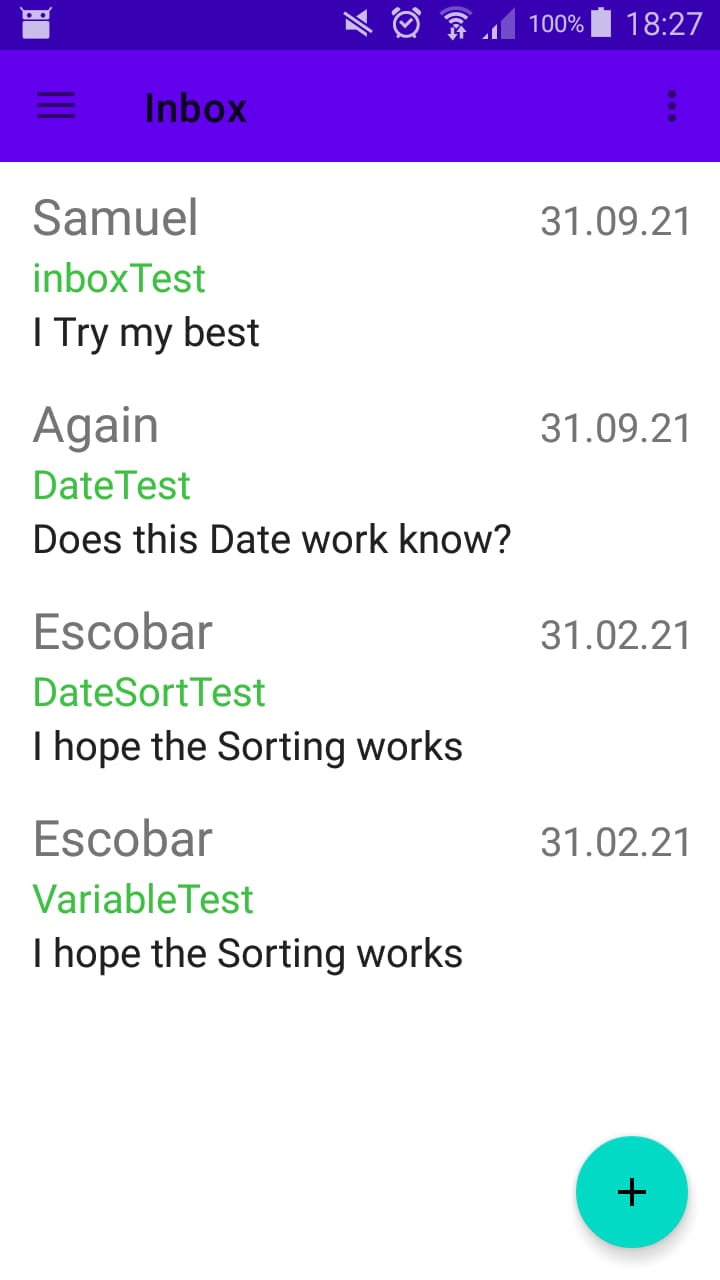
\includegraphics[width=.32\textwidth]{media/inbox.jpeg}
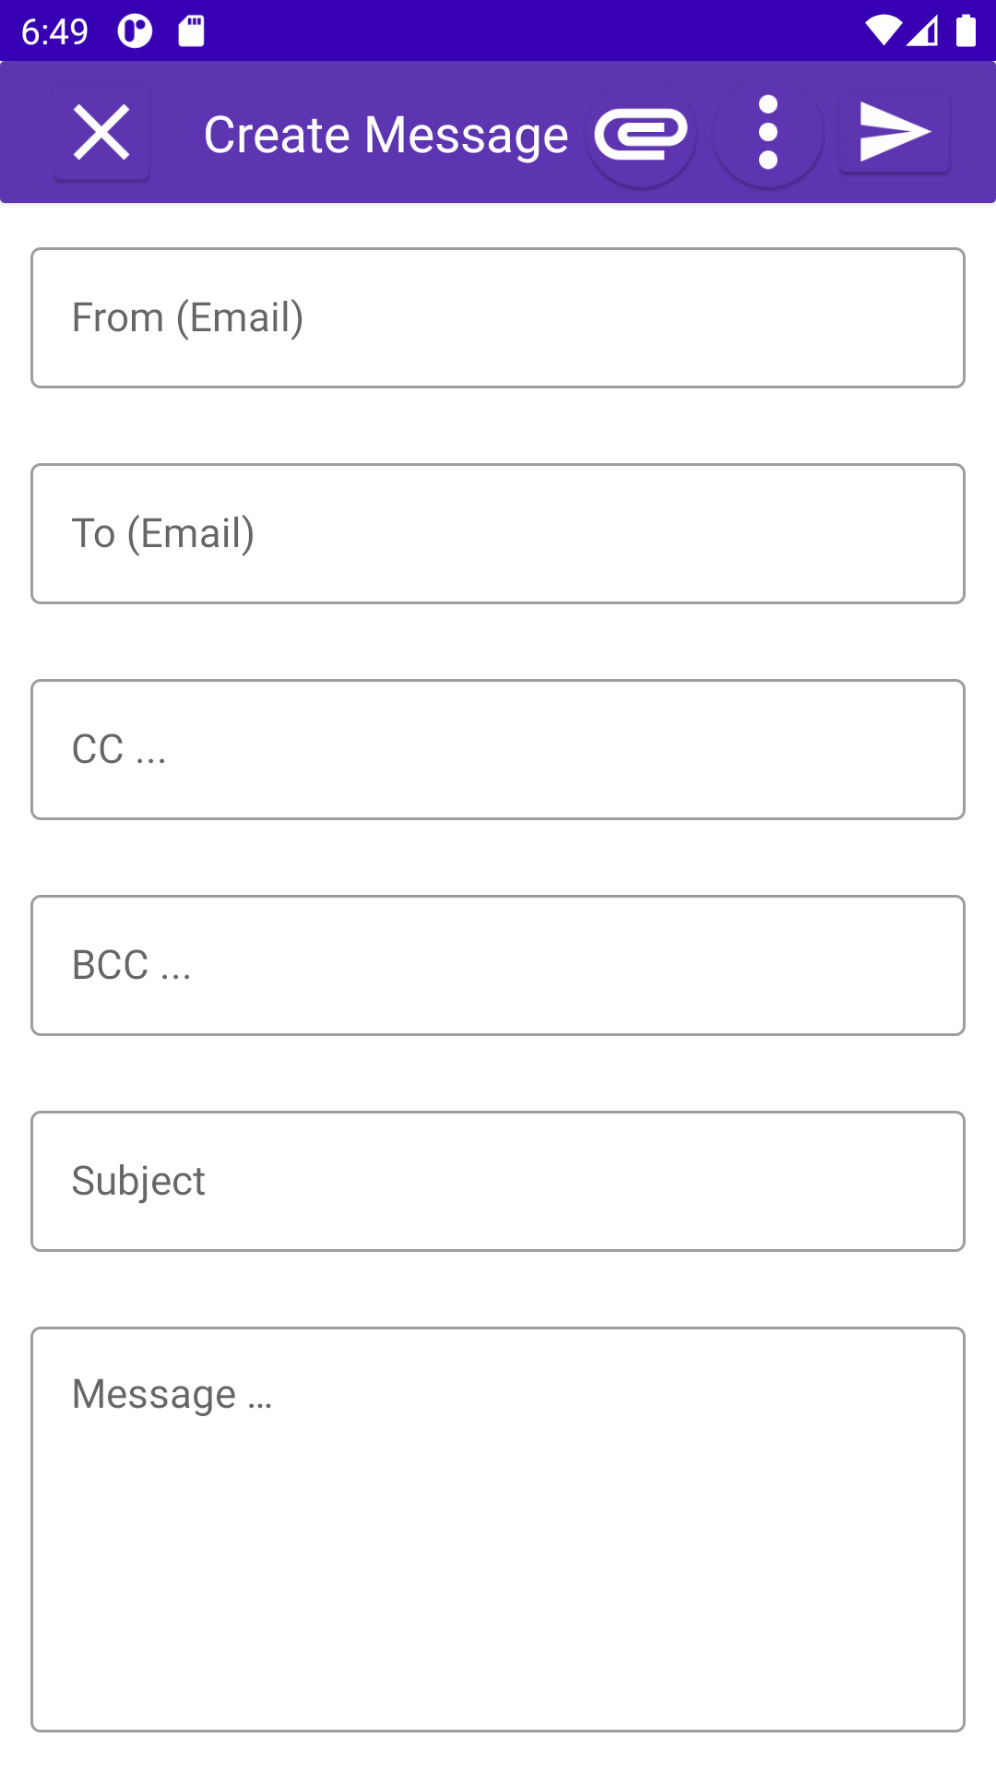
\includegraphics[width=.32\textwidth]{media/fitted-create-message.png}
\caption{die Startup UI von snailmail}

\end{figure}

Wenn man die App startet sieht man als allererstes die durchscrollbare Inbox (siehe mittleres Bild links), hier mit vollkommen arbiträren Testdaten. Bei den 3 Menüpunkten soll im weiteren Laufe der Entwicklung noch die Funktionalität hinzugefügt werden, Emails zu sortieren und durchsuchen.\\

Wenn man im Bild in der Mitte unten rechts das Pluszeichen antippt, erscheint ein Fenster, wo man eine neue Email schreiben kann (Bild rechts). Man kann sie entweder versenden, oder als Entwurf speichern. Wenn der Nutzer sich mit einem Account angemeldet hat, wird die Adresse des Absenders, im Bild entspricht das dem Textfeld mit dem Platzhalter \say{From (Email)}, automatisch mit der aktuellen Email Adresse vervollständigt.\\

Wenn man im mittleren Bild oben links auf das sogenannte \say{Hamburgermenü} drückt, oder wie auf vielen anderen Apps auch von links nach rechts swiped (dt. streicht) erscheint der sog. \say{Drawer} (im Bild links ersichtlich). Dort sieht man den eingeloggten Account, die verschiedenen Mailboxen und ein paar Buttons, um zu den Einstellungen zu gelangen (unten links), einen neuen Email Account hinzufügen (unten Mitte) und um zum Account Manager zu gelangen (durchs tippen auf das Profilbild). Dort kann auf eine andere Mailbox klicken, sodass diese ausgewählt und geöffnet wird.

\subsubsection{Account Management}

Wenn man im Drawer den \textit{Add Email Button} drückt, erscheint ein Pop-up Fenster , wo man seine Anmeldedaten für ein neues Email Konto angeben kann. Da ein Mailserver aber auch von gewissen Standardeinstellungen wie beispielsweise vom standardmässigen IMAP Port 993 (wie definiert von der Internet Society in der IMAP Spezifikation rfc9501 \cite{rfc9501}) abweichen kann, werden in diesem Fenster die zuerst die Standardeinstellungen getestet, indem eine kurze Anfrage an den Server ausgeführt wird. Zuerst wird geschaut, dass nicht bereits ein Account mit der gleichen Email Adresse wie der zu Hinzufügende, wobei dann eine Meldung erscheint für den Nutzer. Dann werden die Anmeldedaten anschliessend mit der Funktion \textit{checkConnection} überprüft, um zu schauen ob man sich mit diesen zum Mailserver verbinden kann.\\

\lstset{language=python}
\begin{lstlisting}
def checkConnection(host, username, password, port):
    try:
        connection = imaplib.IMAP4_SSL(host, port)
        connection.login(username, password)
        connection.logout()
        return True
    except Exception as e:
        print("host: " + host)
        print("username: " + username)
        print("port: " + str(port))
        print(str(e))
        return False

\end{lstlisting}

Wenn die Anfrage erfolgreich ist, werden die Anmeldedaten in der App gespeichert. Wenn nicht, erscheint ein neues Dialogfenster, wo der Nutzer gefragt wird, ob er noch erweiterte Angaben angeben will um die diese dann testen zu können.\\

Wie schon in Punkt 3.2.3 erwähnt, muss man im \textit{Drawer} auf das Profil klicken, umd zum Account Manager zu gelangen wo dann ein Dialogfenster erscheint. Zuerst wird der Benutzer vom Programm angewiesen mit der Nachricht \say{select Account} ein Konto im, wenn man darauf tippt, Drop-Down Menü auszuwählen. Dann kann er eine Aktion ausführen, indem er einer der korrespondierenden Knöpfe drückt, oder mit \say{exit}-Button das Dialogfenster wieder schliessen.\\

\begin{figure}[H]
\centering
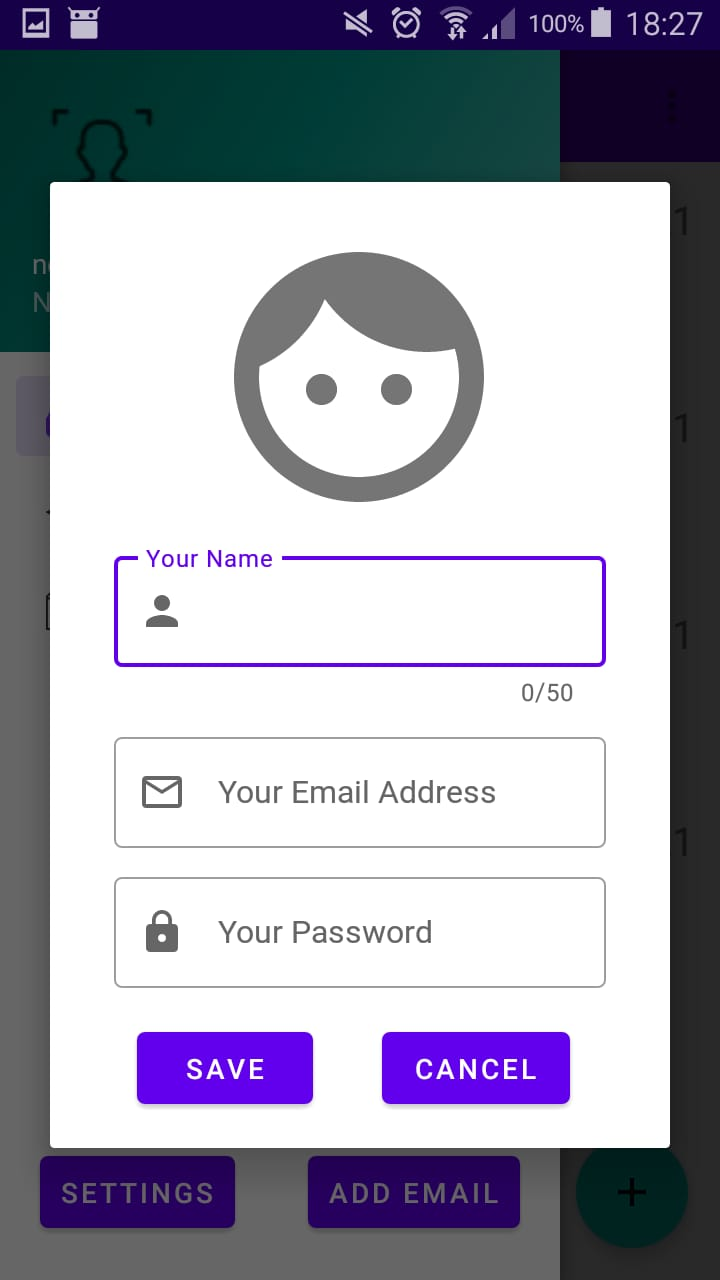
\includegraphics[width=.32\textwidth]{media/plain-add-email.jpeg}
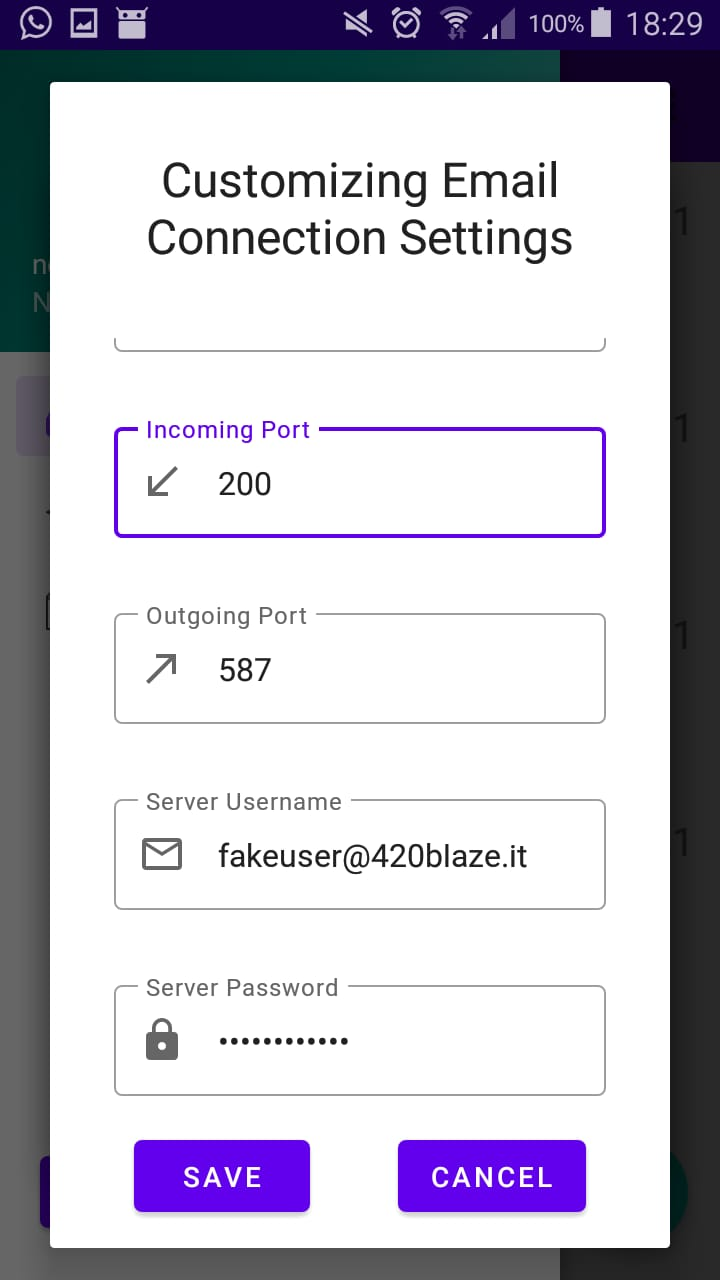
\includegraphics[width=.32\textwidth]{media/advanced-add-email.jpeg}
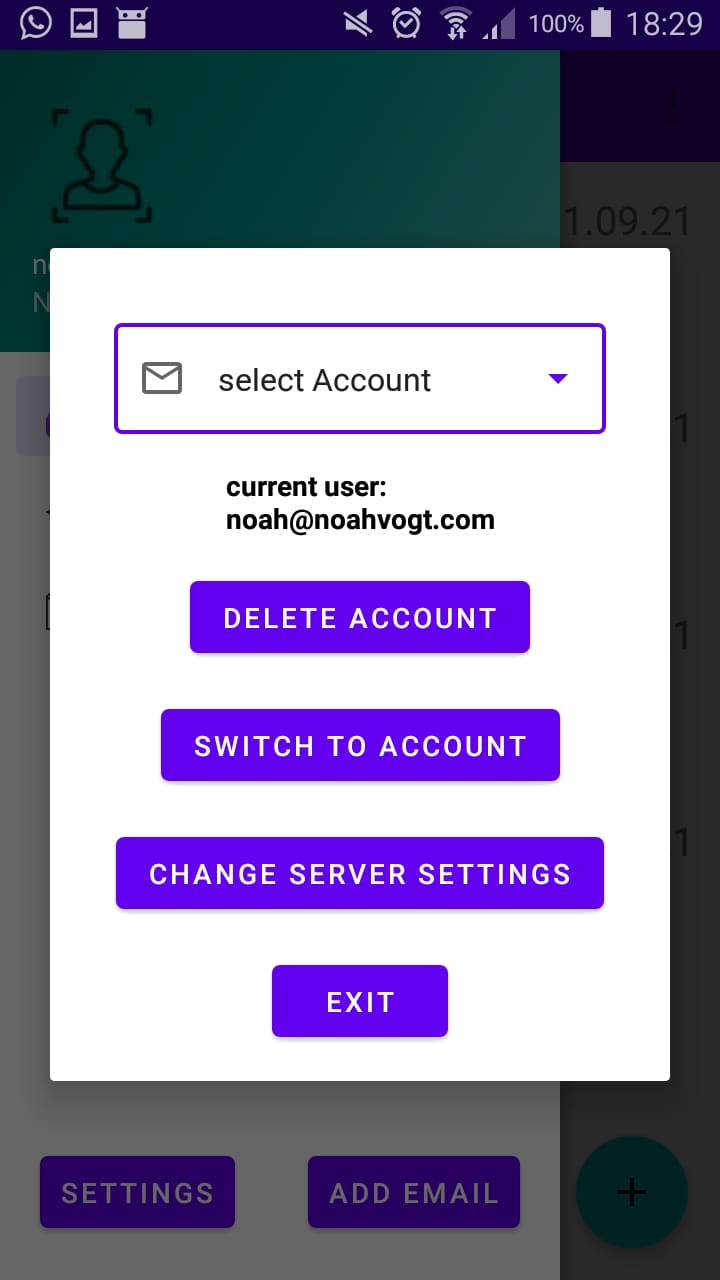
\includegraphics[width=.32\textwidth]{media/plain-account-manager.jpeg}
\caption{das Account Management}

\end{figure}

Der Nutzer kann entweder den ausgewählten Account löschen, zu ihm wechseln, oder seine Server Settings ändern. Beim letzteren erscheint das gleiche Menü wie den erweiterten Einstellungen, um einen neuen Account hinzuzufügen. Wenn der Nutzer seine neuen Mailservereinstellungen speichern will, wird zuerst geschaut, ob die App sich immer noch verbinden kann mit dem Mailserver. Wenn nicht, erscheint eine Fehlermeldung für den Nutzer und die neuen Angaben werden \textit{nicht} gespeichert.\\

Zur Hilfe wir im Dialog des Account Managers die ganze Zeit zur Hilfe den aktuell aktiven Account anzeigt. Nach jeder der Account Manager Aktionen werden immer noch diese Anzeige und die Textfelder im Drawer, wo der Nutzer seinen zur Zeit aktiven Email Account sehen kann, in Echtzeit aktualisiert.


\subsubsection{Recyclerviewer}
% TODO: mehr allgemein erklären

Ein Recyclerviewer ist in fünf grundlegende Teile aufgeteilt. 

\begin{enumerate}

%TODO: dütsch? +Bild
    \item Das recyclerview Objekt, welches ein Container ist und in das User Interface eingebaut wird. 
Es beinhaltet verschiedene Views, welche nochmals unterteilt werden können. In einer View wird in unserem 
Fall eine Nachricht eingebaut mir dem Absender, der Absende Zeit und einem Betreff. 

\end{enumerate}

%\endgroup

\begin{enumerate}

    \setcounter{enumi}{1}
    \item Der Layout manager. Er ist für die form einer einzelnen View verantwortlich. 
Der Layout manager kann auch wieder in drei Arten unterteilt werden. Der Linearlayout Manager sorgt für eine 
Horizontale oder vertikale unterteilung einer View. Hingegen führt der Gridlayout Manager zu einer horizontalen 
und vertikalen Unterteilung des View. Für den Email-Client bietet er die  
beste oberfläche um Nachrichten darzustellen. Es gibt nämlich noch den den Staggeredgridlayout Manager, welcher 
für eine versetzen unterteilung der View kann sorgen. Dies ist aber für eine Email-Client unbrauchbar. 

\begin{figure}[H]
    \centering
    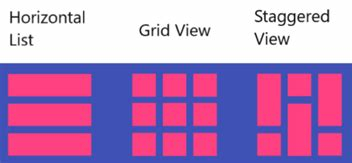
\includegraphics[width=.4\textwidth]{media/RecyclerviewLayoutManagerCropt.jpeg}
    \caption{Layout Manager Recyclerview \cite{LayoutManagerPicture}}
\end{figure}

    \item Der View Holder bietet die Möglichkeit jedes einzelne Raster der View mit einem Item auszustatten mit wiederum einer View in einem Recyclerviewer

    \item Der Adaper ist wohl eines der wichtigsten Teile des Recyclerviewer. Er sorgt für das erstellen des ViewHolder-Objekt und
bindet auch die Daten aus der Database an den View Holder

    \item Die Database ist das Herzstück dieser App und wir auch für den Recyclerviewer verwendet um die 
Views mit den richtig Informationen zu füllen. 

\end{enumerate}

Die Wahl des Layout Manager wurde sehr schnell getroffen. Es war klar, dass eine Nachricht nicht nur eine Information auf horizontaler Ebene anzeigen muss sondern
z.b auch das Datum nicht versetzt angezeigt werden soll. Weshalb der Gridlayout Manager gewählt wurde. Nun hat sich Simon in einem Tutorial über den Recyclerviewer informiert
und konnte sich auch ein beispiel anschauen, woran sich der Recyclerviewer der Email-App zu beginn sehr stark orientierte. \\

% \textbf{https://github.com/android/views-widgets-samples/tree/main/RecyclerView} Recyclerviewer beispiel \\

Nach dem sich Simon über den Recyclerviewer informiert hat, sollte er endlich in das Programm eingefügt werden. Leider gab es da einige Probleme. Der erste Versuch scheiterte daran,
dass die App abstürzte ohne einen Error zu melden. Und nach einiger Zeit war die beste Lösung wieder an einen Punkt zu gehen, an welchem die noch funktionierte, nur ohne vollständigen 
Recyclerviewer. Es dauerte einen ganzen Monat bis eine weitere Version mit Recyclerviewer bereit war. Nur diesmal funktionierte die App. \\

Der Recyclerviewer war an diesem Punkt sehr simpel. Er konnte eine vorbestimmte menge an Views anzeigen, welche in einem Loop generiert wurden, lass die Informationen aus
einer sehr simplen Database aus und er konnte noch nicht aktualisiert werden. Die Informationen konnten nur einmal eingelesen werden und der View-Holder wurde in der gleichen Klasse wie 
der Adapter definiert. \\

Die Database bestand zu diesem Zeitpunkt aus nur einer Klasse, welche fünf Strings definierte, diese einlesen konnte und auch wieder ausgeben konnte. Mit dieser Klasse wurde
ein Objekt erstellt, welches in einer Arraylist, durch einen Loop, eingelesen wurde und jeweils die gleichen fünf Strings überkam. \\

In der Klasse des Adapters wurde durch den ViewHolder die richtigen Textviews ausgewählt, die Views kreiert und mit den Informationen, welche der Adapter bekam, gefüllt. \\

In der Mainactivity wurde dies alles in der onCreate() Funktion ausgeführt, was zur Folge hatte, das der ganze vorgang nur beim Öffnen der App ablieft, da die Funktion onCreate()
nur einmal bei der ersten Ausführung der App aufgerufen wird. So konnte der Recyclerviewer erst nur einmalig mit Informationen versehen werde.

Der CustomAdapter war am Anfang der App dafür zuständig die Daten, welche in einer einfache Klasse abgespeichert wurden, über den 
\textit{Constructor} dem ViewHolder weiter zu geben, welcher dann diese Informationen an eine View im Recyclerviewer band. Im verlaufe der Zeit wurde 
der Adapter angepasst und erweitert. Dies hatte Simon auch sehr grossen Spass gemacht da er auch wirklich alles verstand, jedoch als die Database entstand war der alte 
CustomAdapter überflüssig und wurde ersetzt. Der neue CustomAdapter regelt seine Aufgaben jetzt ein wenig anderst. Zwar viel effizienter mit weniger Code aber nicht 
so Transparent. Der CustomAdapter wird wie der Recyclerviewer in jedem Fragment für den zugehörigen \textit{Folder} neu Aufgerufen und überschreibt den CustomAdapter 
aus der Mainactivity. 

\subsubsection{Input Validation}
% TODO: explain chain of popup windows
\begin{wrapfigure}{r}{5cm}
\centering
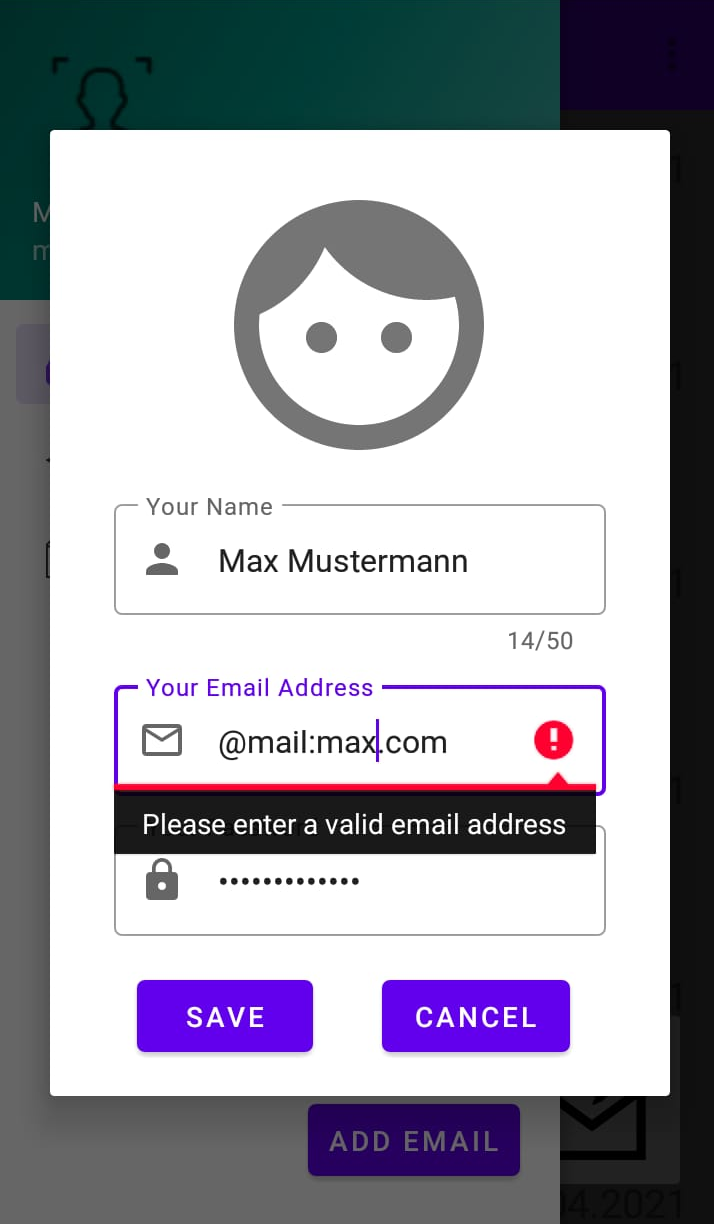
\includegraphics[width=.18\textwidth]{media/inputValidation.png}
\caption{Input Validation}
\end{wrapfigure}

Bei den meisten Textfeldern, wo der Benutzer etwas eingeben kann gibt es in snailmail und es sinnvoll gecheckt werden kann gibt es eine \textit{Input Validation}. Dort wird gecheckt, ob die Eingabe korrekt ist, also ob der Nutzer eine z.B. gütlige Emailaddresse eingegeben hat oder dass er ein Eingabefeld nicht leer lässt. Das Feld mit der falschen Eingabe wird rot markiert und der Nutzer weiss somit, an welcher Stelle er seine Eingabe korrigieren muss. Diese Praxis ist mittlerweile weitverbreitet und auf mobilen graphischen Oberflächen wurde diese von den Autoren als sinnvoll erachtet, weshalb sie auch in ihrer App davon Nutzen gemacht haben.

\subsubsection{Datenbank}

% Nachdem die Grundbausteine für den Recyclerviewer gelegt wurden, war es Zeit eine Database zu erstellen, welche die Informationen der Server 
% Speichern kann, da ein Ziel war POP3 anzubieten. Und mit IMAP muss die geöffnete Nachricht auch einmalig gespeichert werden. Dafür bietet sich eine Dabase gut an.
% \textbf{nicht sicher ob das Stimmt was ich hier schreibe}\\

%TODO: überarbeiten weil in Hauptziel drin
Da viele Daten gespeichert werden müssen, musste eine Möglichkeit her, wie diese möglichst schnell, und der Einfachheit halber mit einer gewissen Abstraktion, in einer sinnvollen Datenstruktur gespeichert werden können. Dazu taugte eine Datenbank für diesen Anwendungszweck und u.a. in Anbetracht der eingrenzenden Umständen, also die Deadline der Arbeitsabgabe, an. Noah hatte schon ein paar wenige Erfahrungen mit Datenbanken, doch da Simon diese Aufgabe übernehmen wollte, las er sich mithilfe eines Buches \cite{riccardi2001} erfolgreich in die Thematik ein.


Ein \textit{relational database management system} ist ein Databasesystem in welchem die Informationen als \textit{tables} gespeichert werden. 
Ein \textit{table} besteht aus Reihen und Spalten. Eine Reihe repräsentiert jeweils ein Object der Database und eine Spalte repräsentiert ein Wert eines Attributes. Im Fall dieser App
gibt es 9 Attribute und einen Objectkey. \\


\begin{tabular}{ |p{1.6cm}  |p{1.1cm} |p{1.1cm} |p{1.05cm} |p{1.15cm} |p{1.15cm} |p{1.25cm} |p{1.75cm} |p{1.25cm} |p{1.15cm}|}
 \hline
 \multicolumn{10}{|c|}{Database Table} \\
 \hline
    ObejctKey &To & cc & bcc & from & date & subject & textContent & folder & seen  \\
 \hline
     01    &Valentin& null & null & Lennard & 01.03.13 & Schule &  Hallo Herr Konrad ...& Draft & true \\
 \hline
\end{tabular} \\

Der Objektkey wird dafür genutzt das Objekt zu identifizieren und aufzurufen. Es können auch weitere dinge mit dem Objektkey gemacht werde. 
Je nach dem wie die Database eingelesen wird, kann am Objektkey festgestellt werden, zu welchem Zeitpunkt eine Objekt erstellt wurde. Bis auf seen und dem ObjektKey sind 
alle Attribute Strings. 

\textit{To} ist das Attribute, welches angibt an wen die Email geschickt werden soll, \textit{From} ist das genaue gegenstück dazu. \textit{Cc} und \textit{bcc} sind die 
Email-Adressen, welche die Emails auch bekommen. Der einzige unterschied ist, dass bei \textit{bcc} diese Adressen nicht einsehbar sind und somit nicht bekannt ist wer diese Email auch liest. 

\textit{Date} gibt das Datum an, an welchem die Email verschickt wurde. \textit{Subject} ist ein Betreff für die Email und \textit{textContent} ist der Text welcher in der Email verfasst wurde. 

Das Attribut \textit{Seen} ist etwas spezieller. Es gibt an ob eine Nachricht von dem Nutzer Gelesen wurde oder nicht. Diese Info wird dann im Recyclerviewer genutzt um die Textart zu verändern
in welcher die Email angezeigt wird. Diese Attribut muss verändert werden, wenn eine Email geöffnet wird. \\

Die Attribute \textit{To}, \textit{from}, \textit{date}, \textit{folder} und \textit{seen} wurden im Databaseconstructor als @NonNull definiert, heisst sie müssen eingelesen werden und können 
nicht null sein. Das macht soweit Sinn, weil eine Email, bis auf \textit{seen}, nicht ohne diese Angaben versendet werden können und ohne zu wissen in welchem Ordner die Email einzuordnen ist,
kann die Email auch nicht richtig angezeigt werden. \\

Als letztes gibt es noch das Attribut \textit{folder}, es gibt an, von welcher Art die Email ist. Es gibt in der App fünf Ordner. Sie heissen \textit{Draft}, \textit{Sent} 
\textit{Inbox}, \textit{Spam} und \textit{Archive}. Die Database kann nach einzelnen Attributen ausgelesen werden. So können die Emails mit den richtigen
folder Attributen, in den richtigen Ordnern angezeigt werden. Jeder Ordner hat sein eigenes Fragment, welches aufgerufen wird, wenn der Ordner ausgewählt wird.
Wenn ein solches Fragment aufgerufen wird, wird auch die Database mit den richtigen Befehlen neu ausgelesen.  \\


%Für Android gibt es nicht viele Sprachen um eine Database zu erstellen. Die bekannteste ist SQLite .Jedoch ist SQLite nicht sehr simple und es kann sehr komplex werden, wenn
%die Database bis auf bytes genau Programmiert werden soll. Ebenfalls lag es nicht im Zeitplan eine weitere Programmiersprache zu lernen. Nach kurzer 
%recherche stellte sich heraus, dass es eine Library gibt, welche den Umgang mit SQLite vereinfacht und diese sogar mehr Sicherheit bietet.\\



\begingroup
\setlength{\intextsep}{10pt}
\setlength{\columnsep}{15pt}

\begin{wrapfigure}{r}{8cm}
    \centering
    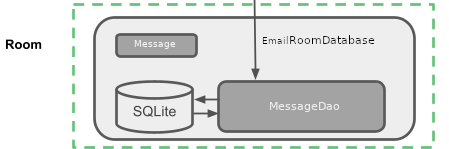
\includegraphics[width=.4\textwidth]{media/RoomStructure.png}
    \caption{Room Struktur \cite{appStructurePicture}}
\end{wrapfigure}


Room ist eine Art Schicht über der SQLiteDatabase. 
Room besteht grundsätzlich aus drei Teilen. Die Database dient als Hauptzugriffspunkt für die gespeicherten Daten der App. Sie ist mit @Database markiert. 
Eine \textit{Entity} repräsentiert einen \textit{table} in der Database und die \textit{DAO} Klasse beinhaltet die Methoden um auf die Database zu zu greifen. Sie kommuniziert
mit SQLite um de Zugriff auf die Daten zu ermöglichen \cite{roomStructure}


\paragraph{MessageDao}

In der \textit{DAO}-Klasse können SQL statements verwendet werden. Um auf die Database zu zugreifen und nur Gewisse 
Objekte zu erfassen, hat Simon ein paar wenige SQL statements gebraucht. SQL ist zum Glück in diesem Fall sehr selbsterklärend, 
dennoch werden wir darauf eingehen.\\


\lstset{language=SQL}
\begin{lstlisting}
    /* get Draft messages*/
    @Query("SELECT * FROM message_table WHERE folder LIKE 'Draft' ORDER BY date ASC")
    LiveData<List<Message>> getDraftMessages();
\end{lstlisting}

\textit{Querys} sind anfragen an die Database nach Informationen. Sie können auf verschiedene \textit{tables} zugreifen und Informationen abgleichen und auswählen. 
In einer DAO von Room werden die SQL-statements mit @Query markiert. SELECT heisst, dass etwas ausgewählt werden soll und mit * ist gemeint alles. Mit FROM wird angegeben von 
welchem table, in diesem Fall vom message\_table. Mit WHERE können Spalten der Entity ausgewählt werden. Hier wird die \textit{folder} Spalte 
gewählt um mit LIKE ein Attribut zu bestimmen. So wird nun ein Attribut namens 'Draft' gewählt. Mit ORDER By kann die Ausgabe noch sortiert werden. So wird die Ausgabe anhand der Spalte 'date'
aufsteigen Sortiert. \cite{queryExpl}

\subsubsection{Repository/ViewModel}

\begingroup
\setlength{\intextsep}{1pt}
\setlength{\columnsep}{4pt}

\begin{wrapfigure}{r}{5.5cm}
    \centering
    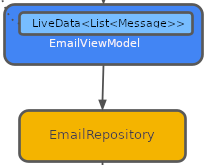
\includegraphics[width=.4\textwidth]{media/ViewModelRepository.png}
    \caption{EmailViewModel and Repository
    \cite{appStructurePicture}}
\end{wrapfigure}

Mit der Database wurden auch ein Repository und ein Viewmodel mit Viewholder erstellt. 
Das Repository verwaltet die Datenquellen. Im Normalfall würde es Daten von einem Server verwalten und in die Database einlesen. Ebenfalls kann
es auch Daten die der User direkt eingibt einlesen. Zwar nicht direkt von der Activity aber über ein Viewmodel können Daten in die Database eingelesen werden. Das Repository 
stellt dazu die Funktionen für das Viewmodel zur Verfügung. 
Da in diesem Falle keine anständige Java Library gefunden wurde, welche nicht uralt oder eine Dokumentation zur Verfügung hatte mussten die Daten vom Server mit einer 
Python Library eingelesen werden. Noah Programmierte dazu in Python mit einer Library ein Programm welches die Daten von eine Server herunterlädt und in die Database einliest. 

In diesem Falle das EmailViewModel, stellt Funktionen zur Verfügung, mit welchen auf die Database, über das Repository, zugegriffen werden kann. Ebenfalls gibt es LiveData zurück 
mit welcher die Mainactivity die observer Verknüpfungen erstellen kann. Mit dem ViewHolder in diesem Fall dem EmailViewHolder können Daten an View gebunden werde. In dem Fall wäre das 
der Recyclerviewer.
So wird die Mainactivity informiert, wenn eine Änderung der Database vorgekommen ist. Im Fall dieser App wird zwar 
ein Recyclerviewer in der Mainactivity mit Observer und Adapter erstellt, jedoch wird dies nur gemacht um das gleiche für jedes Fragment zu machen, welche dann den Recyclerviewer und den 
observer aus der Mainactivity überschreiben. Die einzelnen \textit{Folder} haben jeweils ein Fragment zugeordnet, in welchen der einzige unterschied ist, dass sie andere 
Attribute aus der Database abfragen um die den \textit{Folder} entsprechenden \textit{Messages} zu bekommen. 

An diesem Beispiel ist es vielleicht leichter zu verstehen. Dies ist die Funktion welche an einer Variable vom Typ EmailViewModel ausgeführt wird. In dem Fragment HomeFragment in der
onCreateView Funktion, welcher immer ausgeführt wird wenn dieses Fragment aufgerufen wird. 


\lstset{language=java}
\begin{lstlisting}
        mEmailViewModel = new ViewModelProvider(this).get(EmailViewModel.class);
        mEmailViewModel.getInboxMessage().observe(getViewLifecycleOwner(), messages -> {
            /* Update the cached copy of the messages in the adapter*/
            adapter.submitList(messages);
        });
\end{lstlisting}

Die Funktion getInboxMessage() is im der Klasse EmailViewModel definiert und gibt LiveData<List<Message>> zurück, was soviel ist wie eine Liste der Objekte in der Database, eingebettet 
in LiveData.

\lstset{language=java}
\begin{lstlisting}
    public LiveData<List<Message>> getInboxMessage(){ return mInboxMessage;}

\end{lstlisting}

\lstset{language=java}
\begin{lstlisting}
        private LiveData<List<Message>> mInboxMessage;

        public EmailViewModel(Application application) {
        super(application);
        mEmailRepository = new EmailRepository(application);
        mInboxMessage = mEmailRepository.getInboxMessages();
        }

        public LiveData<List<Message>> getInboxMessage(){ return mInboxMessage;}

\end{lstlisting}


\lstset{language=java,numbers=none}
\begin{lstlisting}
    private LiveData<List<Message>> mInboxMessage;

    public EmailRepository(Application application) {
        EmailRoomDatabase db = EmailRoomDatabase.getDatabase(application);
        messageDao = db.messageDao();
        mInboxMessage = messageDao.getInboxMessages();
    }

        public LiveData<List<Message>> getInboxMessages() {
        return mInboxMessage;
    }


\end{lstlisting}

Im \textit{Cunstroctor} von dem EmailViewModel wird der Variable mInboxMessage die Daten aus dem Repository übergeben welche diese wieder im \textit{Constructor} von dem MessageDAO überkommt.


\subsubsection{Draft Messages}

\begingroup
\setlength{\intextsep}{1pt}
\setlength{\columnsep}{4pt}


\begin{wrapfigure}{r}{9cm}
    \centering
    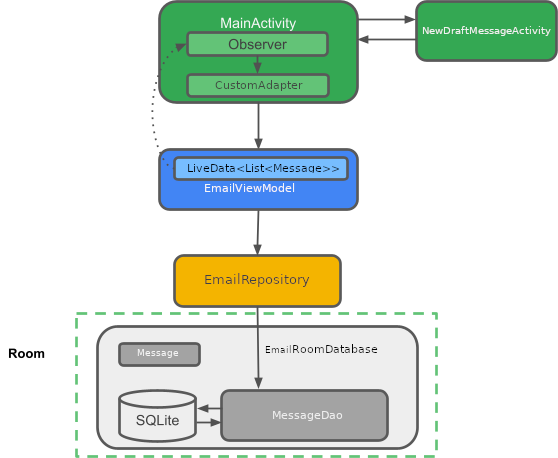
\includegraphics[width=.55\textwidth, height=.55\textwidth]{media/AppStructure.png}
    \caption{App Structure \cite{appStructurePicture}}
\end{wrapfigure}

Der ganze Aufbau der in den Kapitel von vorhin erklärt wurde, hatte nur zwei Ziele. Einmal das einlesen von Emails von einem Server und das Einlesen von Emails
über ein Fragment genannt messageCreateFragment. Diese Fragment interagiert mit einer Activity genannt NewDraftMessageActivity. Die Mainactivity startet beim Klicken auf einen Button 
das messageCreateFragment. Dieses liest die Daten ein welche der User in das Fragment schreibt und übergibt sie mit Hilfe der NewDraftMessageActivity direkt an die Message Klasse und somit in die 
Database.  \\

Dies ist der grobe Aufbau um Messages anzuzeigen. Wenn etwas durch die NewDraftActivity verändert wird, wird der Observer informiert, welcher den CostumAdpater informiert und bis nach 
ganz unten die neuen Informationen ausliest.

%TODO: alles um de Server mit Python und repository etc. Dänkfähler mit Aktualisierung vo de Ordner
\subsubsection{Server Connection}

\begin{figure}[H]
\center
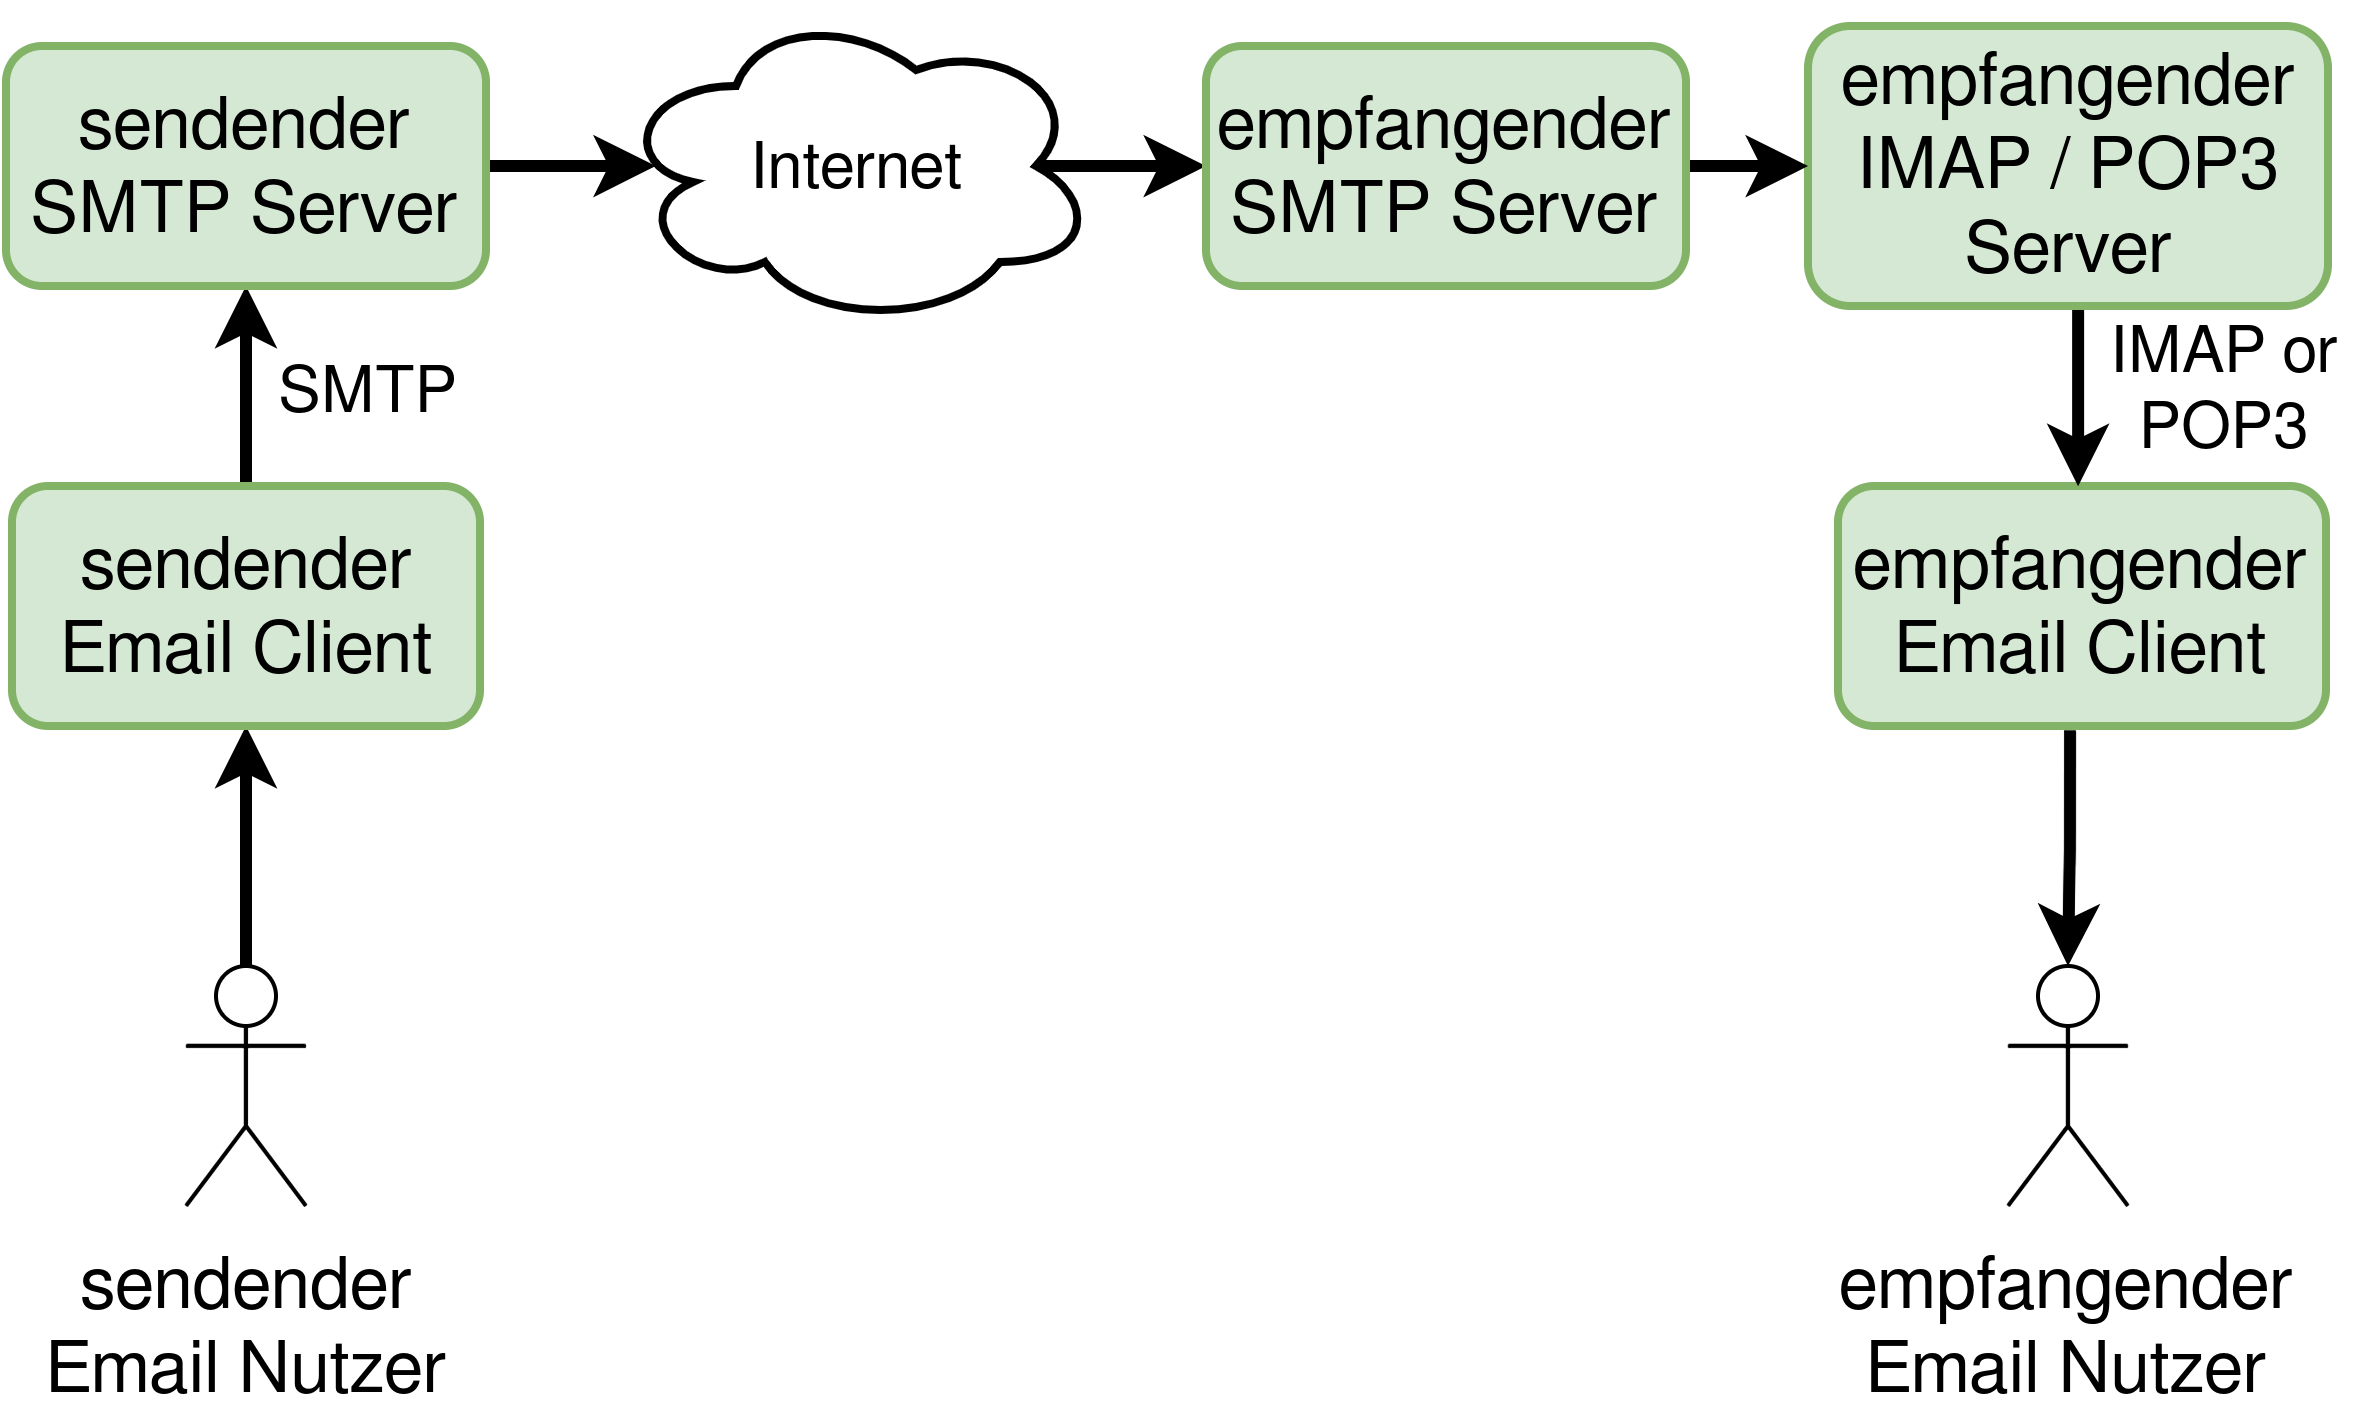
\includegraphics[width=.7\textwidth]{media/connection-diagram.png}
\caption{Diagramm Email Versand}
\end{figure}

\phantom{.} \\ % hack to fix line wrapping in the next paragraph
Vereinfacht funktioniert der Versand von Emails wie im obigen Diagramm: Ein Nutzer der eine Email versenden will interagiert mit seinem Mail Client und gibt durch ihn den Befehlt die Email zu versenden. Der Email Client verschickt die Mail an den SMTP Server des sendenden Nutzers, wo dieser zum SMTP Server des empfangenden Nutzers gelangt, von dort aus zu seinem IMAP oder POP3 Server. Wenn der Mail Client des Empfängers eine Anfrage an seinem SMTP / POP 3 macht, kann er diese einlesen und der Nutzer kann nun seine neue Email lesen.\\

Das Versenden von Mails wird in der App einzeln gemacht: Für jede zu sendende Email wird die Funktion \textit{sendStarttls} (siehe folgend) aufgerufen. Zuerst wird der der SSL Kontext initialisiert, dann werden die Angaben der Mail zu einer korrekt kodierten und formatierten Nachricht umgewandelt und schliesslich mit der \textit{smtplib} Bibliothek versendet.

\lstset{language=python}
\begin{lstlisting}
def sendStarttls(host, sendingMail, receivingMail, password, message="",
                 subject="", port=587, cc=[], bcc=[]):
    context = ssl.create_default_context()

    if type(cc) is not str:
        cc = ",".join(cc)
    if type(bcc) is not str:
        bcc = ",".join(bcc)
    utf8Message = ("Subject: " + subject + "\nCC: " + cc + "\nBCC: " + bcc +
                   "\n\n" + message)
    decoded = utf8Message.encode('cp1252').decode('utf-8')

    with smtplib.SMTP(host, port) as serverConnection:
        serverConnection.starttls(context=context)
        serverConnection.login(sendingMail, password)
        serverConnection.sendmail(sendingMail, receivingMail, decoded)
\end{lstlisting}

\subsection{Umsetzung}
\subsubsection{Bugs}
% Erklärung woher, warum falsch, wie gelöst
Programmierfehler schleichen sich in jedem Softwareprojekt ab einer gewissen Komplexitätsstufe ein. Damit hatten auch die Entwickler diese Projektes zu kämpfen. Hier dazu ein kleines Beispiel:\\

% GUI stuff -> oneliner commit 
Als der RecyclerViewer das erste Mal eingebunden werden konnte, ohne dass die App nach dem Öffnen direkt abstürzt, war aber das Problem, dass am oberen Teil Inhalte abgeschnitten waren. Das konnte gelöst werden, indem diese Codezeile in der Datei \textit{app/src/main/res/layout/activity\_main.xml} an der richtigen Stelle eingefügt wurde:

\lstset{language=XML}
\begin{lstlisting}
android:paddingTop="50dp"
\end{lstlisting}

\subsubsection{Probleme / Hiccups}
% RecyclerViewer, shit java IMAP libraries
Probleme waren die unnötig vielen Layouts, welche entstanden bei unserer App. Vielleicht hätten diese minimiert werden können, wenn die Entwickler eine siginfikant höhere Erfahrung im Bereich der Android Entwicklung hätten, oder wenn die verschiedenen Inhalte beim Aufrufen weniger Layouts generieren würden, oder diese könnten besser wieder referenziert werden.\\

Mit gewissen Biobliotheken sind auch Probleme entstanden, dazu wird später in diesem Text noch das Problem mit den Email-Bibliotheken geschildert.

\subsubsection{Kommunikation}

Die Menge an Kommunikation hat sich eingependelt zwischen den Anforderungen, Bedürfnissen und sozialen Kapazitäten der beiden Autoren. Einer wollte eher etwas mehr Dialog, der andere weniger. Das gegenseitige Vertrauen war aber auch soweit vorhanden, dass man sicher ziemlich sicher sein konnte, dass der andere gewisse abgemachte Zeiten einhält und Nachrichten nicht unnötig lange unbeantwortet lässt.\\

Es konnten auch gute Strukturen für die Kommunikation geschaffen werden, so wurde eine \textit{diary}, also eine Art Tage- oder Logbuch verwendet, um den Arbeitsprozess zu dokumentieren, was sich insbesondere bei den Anfängen des Projektes als nützlich herausstellte. Auf diesem Dokument und der \textit{Git Commit History} basiert die Dokumentation dieser Arbeit.\\

Sowohl im Programm-Quellcode der App als auch im Quellcode dieser Arbeit haben die beiden Autoren Notizen in Form von Codekommentaren gemacht - teilweise sich sogar gegenseitig- voll nach dem Motto: \say{Hey, kannst du das dann dort noch einfügen? Du kannst das ja besser als ich.}\\

Auch haben sich die beiden zeitweise Montags zusammen hingesetzt und den Arbeitsprozess in dieser Weise zu besprechen und um sich die nächsten Aufgaben zu verteilen.\\

Insgesamt verlief die Kommunikation doch reichhaltig, obwohl einer der beiden Autoren doch etwas überdurchschnittlich schwer digital erreichbar ist. Die grobe Aufteilung des Programmes um daran zu entwickeln um dann die Komponenten wieder zusammenzufügen hatte etwas von dem typischen Modularität und des Touches der Linuxphilosophie.
% TODO: bruche mir de satz mit de 'linuxphilosophie' @simon? weiss grad iwie nid

\subsubsection{Namensfindung}
Für die App musste auch noch ein Name her, doch die allerlängste Zeit hatten die beiden Autoren entweder keine Idee oder der Name wurde schon von einer anderen App verwendet. Doch als einer der beiden Autoren seinen Vater fragte nach Namensideen, war einer der Vorschläge \say{Schneckenpost}. Dies ist natürlich eine offensichtliche ironische Anspielung darauf, dass unsere App schneller sein soll als die meisten Apps. Doch da ein englischer Name erwünscht war, wurde es einfach direkt übersetzt in \say{snail mail}. Nun war nur noch die Frage, wie man es darstellen sollte, etwa \say{SnailMail} (CamelCase), \say{snailMail} (mixedCase), \say{Snail Mail}, \say{snail mail} oder \say{snailmail}. Es wurde sich für das letzte entschieden, da dies das wichtigste Designkonzept der App am besten wiederspiegelt: Die Einfachheit. Gleich wie die App lautet auch übrigens der Name des GitHub Repositorys der App:\\

\url{https://github.com/noahvogt/snailmail}

\subsection{Testing}
% TODO: provide testing data + text

\section{Resultate}
\subsection{Vergleich mit unseren ursprünglichen Zielen}
Das User Interface ist erfreulich gut im Einklang mit den ursprünglichen Zielen, es ist wirklich simpel rausgekommen ohne irgendwelchen unnötigen Schnickschnack. Simpel is das GUI also, doch wie steht es mit der Bedienbarkeit? Dazu haben wir Freunde und Bekannte eingespannt, ihnen ein Handy mit der App in die Hand gedrückt und gesagt sie sollen einen Mailaccount einrichten um dies herauszufinden. Dabei haben sich die meisten gut und schenll zurechtgefunden, obwohl die App ja noch nicht fertig ist.\\

Die App selber ist wie von uns in den Zielen vorgegeben Free Software. Doch erst es wurde herausgefunden, dass die von diesem Projekt verwendete \say{chaquopy} Bibliothek aber proprietär ist, und somit indirekt ein Konflikt mit den ursprünglichen Zielen: Es wurde zwar nicht expilizit angegeben, dass die alle Bibliotheken zwingend auch Open Source sein sollen, doch es ist nicht im Sinne eine nichtfreie Library zu haben. Im Laufe der weiteren Softwareentwicklung wird dieser Fehler noch unbedingt behoben werden müssen. Dieser Misstand ist auch teilweise dem Dependencymanagement von Gradle anzulasten, da dieser immer nur die binäre Version herunterlädt und der Source Code von Dependencies nirgends gescheit verlinkt ist.\\

Die wichtigsten Funktionen der App wurden erreicht, man kann Emails schreiben, lesen, hat verschiedene Mailboxes getrennt ansehen und man kann seine Email Accounts gut managen, also hinzufügen, ändern und entfernen. Doch gewisse Features, nämlich Pushnachrichten, Suchfunktionen, HTML output parsing, ein visuelles Atribut, wo man sieht ob eine Nachricht gelesen wurde in der Mailbox fehlen noch ganz und Funktionen wie die Einstellungen, das synchronisieren der Datenbank mit dem Mailserver und die Anhangfunkionalität sind noch nicht fertiggestellt und es gibt auch noch gewisse Bugs bei der Entstehung von \say{edge cases} \cite{edgecase} bei bestimmten, einzelnen Emails.\\

Ursprünglich wurde zusätzlich ein Pluginmanager - dabei angelehnt an die Funktionsweise von vim-plug\cite{plug} - geplant einzubauen, doch diese Idee wurde mittlerweile verworfen, da es als weitaus sinnvoller und effizienter angesehen wurde von den Autoren einfach klassische Patches zu verwenden für solche Dinge ähnlich wie dies bei der suckless.org Software \cite{dwm}.

\subsection{Vergleich mit der Konkurrenz}
Es ist gar nicht so einfach diese App zu vergleichen mit ihrer Konkurrenz, da sie ja noch nicht fertig entwickelt ist. Aus diesem Standpunkt heraus vergleichen wir nur die fertigen Funktionen mit der Konkurrenz.\\

Im Vergleich mit der Konkurrenz sticht sie heraus durch ihre simple Art, so wie das geplant war. Die Funktionalitäten sind dabei auch wesentlich rüdimentärer, oder besser gesagt mehr \say{suckless} als die der Konkurrenz. Die Farben und das Layout des User Interface sollte zwar simpel sein, doch das visuelle Zusammenspielen von Farben und dem Layout haben gewisse Konkurrenzprodukte, welche immerhin auch von Fortune 500 Unternehmen entwickelt werden, zweifelsohne besser umgesetzt als die Autoren dieser App.
\subsection{Vor- und Nachteile unserer App}
\subsubsection{Pro}
Für die Nutzung der App sprechen simple Nutzeroberfläche und Codebasis, welche nach Fertigstellung der initialen Entwicklung eine der besten simplen Email Client werden sollte.
\subsubsection{Kontra}
Dagegen sprechen, dass gewisse Funktionen welche laut den Autoren nicht in einen Emailclient gehören nicht vorhanden sind, wie beispielsweise die Funktionalität RSS Feeds zu lesen, wie es der allseits bekannte Mailclient \cite{thunderbird}.

\section{Selbstreflexion}

\subsection{Was Gut Lief}
% komm., vcs, java syntax (allg.)
Das Arbeiten mit \textit{Git} als \textit{Version Control System} verlief gut und half ihrer Meinnung nach enorm beim Arbeitsprozess und dessen Strukturierung. Mit der Syntax der verwendeten Programmier- und Markupsprachen Java, Python und XML konnte gut umgegangen werden, obwohl die beiden noch recht wenig Erfahrung mit Java hatten. Die Codestruktur fanden sie den Umständen entsprechen gut und sinnvoll.
\subsection{Was Schlecht Lief}
% ******* java shit tier libraries
Dass es keine mit Gradle funktionierede, ausreichend dokumentierte und/oder nicht veraltete IMAP- und Emailbibliotheken für Java. Deshalb wichen wir auf die um Welten besser funktionierende Pythonbibliotheken \textit{imap} und \textit{emaillib} aus. Dazu mussten wir eine Library namens \textit{Chaquopy} benutzen, um Python als Bytecode kompiliert in unsere Java App einbauen zu können. Das ist natürlich unschön, aber die Funktionalität wär halt die oberste Priorität.\\

Etwas das nicht direkt schlecht lief aber sehr viel Zeit brauchte ist, dass wenn ich (Simon) zum Beispiel eine Database für den Recyclerviewer gemacht habe, zwar nur eine Testversion, 
ich diese im späteren verlauf komplett überarbeiten durfte. Es war zwar nur eine Testversion aber dass diese so weit von einer professionelle Database entfernt war, war mit nicht klar. 
In so einer Situation war ich nicht nur bei der Database. Mit dem Recyclerviewer hatte ich solche Probleme sogar öfters. Oft hat zwar noch nicht viel funktioniert aber ich musste den Recyclerviewer
öfters komplett umschreiben. Als ich die erste Version hatte, hatte ich eine sehr simple version einer Database und durch dies hat sich auch ein simpler Adapter entwickelt. 
Aber diesen konnte ich mit der Zeit sehr gut an de Recyclerviewer anpassen. Ich habe ihn auch sehr stark ausgebaut. Als ich jedoch eine vollstendige Version einer Database hatte, musste ich den 
Adapter so gut wie löschen. Solche Dinge haben den Arbeitsprozess sehr stark ausgebremst und die Arbeit begann mich zu nerven, da teilweise klar war, dass ich das was ich gerade
mache sowieso nochmals überarbeiten muss. 

\subsection{Was Wir Gleich Machen Würden}
% As long as java is not deprecated in the future for android programming, we would still use it as it is the most ``native'' way of programming. The new java clone/fork of google, Kotlin, would be a worse choice in our eyes, as your are even more dependent on google code, which you are already by using android.
Wenn wir diese in die Vergangenheit reisen könnten und die App von Neuem machen könnten, würden wir am Userdesign nichts ändern, und auch weiterhin mit \textit{Git} als \textit{VCS} arbeiten und für jedes noch nicht einsatzbereite Feature einen neuen \textit{Branch} machen. Die Arbeitsweise an sich hat sich aus unserer Sicht bewährt und ist ein passabler Weg, kollaborativ an einem Softwareprojekt zu arbeiten.
\subsection{Was Wir Anders Machen Würden}
% As java is much slower than language that can be compiled into native binaries we would try to use more C or C++ libraries to improve speed and portability.

Code der in Java geschrieben wurde, kann nicht nativ auf einer Maschine laufen, sondern muss durch eine virtuelle Maschine, die \textit{Java Virtual Machine (JVM)} während der Ausführung in nativen Code umgewandelt werden. Deshalb würde bei einem Rewrite wohl besser mehr Code in C oder C++ geschrieben werden, um die Geschwindigkeit und Portabilität zu erhöhen. Java komplett wegzulassen ist aber weder vorgesehen noch praktisch sinnvoll umsetzbar. \\

Uns ist öfters gesagt worden, dass das managen der Zeit sehr wichtig ist. Wir sind davon ausgegangen, dass wir dies auch gut eingeplant haben. Dem war leider nicht so und wir 
würden uns mehr gedankten machen beim Planen wie auch, wie lange wir an einem Problem arbeiten bevor wir das Feature entfernen, als das wir sehr lange daran arbeiten. 


% use more c libs for speed and less java
\subsection{abschliessende persönliche Schlussfolgerung}
Wir haben das Gefühl, einen guten ersten Einblick in die native Android Programmierung mit Java und Python bekommen zu haben. Wir haben uns vertraut gemacht mit den Vorzügen aber auch Nachteilen dieser Art von Programmierung und der Plattform Android.\\

Wir sind zwar etwas enttäuscht, dass wir nicht alle geplanten Ziele erreicht haben, doch wir haben noch genug Motivation die App in den nächsten paar Wochen und Monaten fertigzustellen. Denn die Arbeit hat uns insgesamt doch gefallen, trotz einigen Motivationstiefs, sodass wir auch gerne unseren Freunden und Familie von ihr erzählt haben.\\

Was uns auch noch sehr gefallen hat ist das Arbeiten mit dem Version Control System \textit{Git} und der Plattfrom \textit{Github}, denn so konnte man gut den Fortschritt sehen und tracken, schliesslich machte das kollaborative Arbeiten an einem Projekt dieser Grösse besonderns Sinn und konnte gut Nutzen machen von der Funktionalität dieses Systems.

\section{Danksagung}
Wir (Simon und Noah) möchten uns bedanken bei unserer Betreuungslehrperson Dr. Viktor Yakonthov, und unserem Koreferenten D. Bühler bedanken, dass sie uns die Arbeit erlaubt haben durchzuführen und ihre Bereitschaft, zu Helfen bei allfälligen Fragen.

\clearpage
\printglossary

\newpage
\printbibliography
\end{document}
